\documentclass[../../main.tex]{subfiles}

\begin{document}

\chapter{Supplementary information for Chapter 2}
\label{ensemble-inference-si}

\begin{refsection}

	This supplement presents the theoretical underpinnings for the kinematic ensemble representation and its efficient implementation, covering the following concepts:
	1) group theory for kinematics,
	2) Hilbert spaces of functions,
	3) orthogonal bases in these spaces,
	4) the generalized Fourier transform from harmonic analysis on the kinematic groups,
	5) the diffusion normal distribution,
	6) the kinematic ensemble representation,
	7) simulating data from the kinematic ensemble, and
	8) notes on implementing the method.

	As these topics span several disciplines, we do not attempt to exhaustively address these concepts.
	Instead, we focus only on details that are either necessary for the proofs contained herein or aid in developing a conceptual understanding of the method.
	Much of these details are classical results included for completeness or to ensure consistency of conventions and assumptions.
	A more formal and detailed introduction to these concepts can be obtained by studying the included references.
	Where necessary, we have included detailed proofs that we have not seen in the literature.

	\section{Group theory for kinematics}\label{manifolds}

	Kinematics deals with the motion of geometric objects.
	This discussion is limited to rigid body kinematics, which concerns the shape-preserving transformations comprised of translations, rotations, and their composition, motions.
	Though we have an intuitive understanding of the kinematic motions, for the purposes of computation, it is necessary to formally introduce them and their properties.
	Rotations, translations, and motions are all examples of groups.
	Before introducing groups, we need to introduce the concept of a manifold.

	\subsection{Manifolds}\label{manifolds}

	A $d$-dimensional manifold is a topological space that locally looks like $\bbR^d$, the $d$-dimensional real (Euclidean) space.
	That is, we can describe any point with some $d$-dimension coordinate system.
	We are not necessarily able to describe every point with the same coordinate system;
	rather, we only require that every point is in a neighborhood that can be described in a coordinate system.

	Such a coordinate system is more precisely defined as a chart, an invertible map that takes every point in some neighborhood on the manifold to a subset of $\bbR^d$.
	A collection of charts that covers the entire manifold is called an atlas\footnote{
		These terms are not coincidental;
		one familiar example of a non-Euclidean manifold is the 2-sphere $\mathbb{S}^2$ (the usual sphere embedded in three dimensions), to which Earth is topologically identical.}.

	We call a manifold smooth if the maps associated with the charts are differentiable.
	On a smooth manifold, we can smoothly transition from one set of coordinates to another set of coordinates for the same point \supercite{leeIntroductionSmoothManifolds2003}.
	Because this composed map is from $\bbR^d$ to $\bbR^d$, we can use the familiar machinery of calculus that is defined in real spaces on these far more complicated nonlinear spaces.

	\subsection{Tangent spaces}\label{tangent-spaces}

	Every point on a smooth manifold has a tangent space.
	The tangent space at a point is the vector space\footnote{
		A vector space is a space whose elements are vectors; that is, they can be added, and they can be scaled by multiplication with a scalar number.}
	containing all tangent vectors to all possible curves passing through that point.
	For example, on the sphere, we could picture the tangent space at a point as the plane exactly tangent to the sphere at that point.
	The tangent spaces of nearby points have no relationship to one another without endowing the manifold with more structure.
	We can intuitively think of tangent vectors as velocity vectors; indeed, we will see later that angular velocities are members of a particular tangent space to the manifold of rotations.

	We write the tangent space at a point $p \in M$ as $T_p M$, so that all $X \in T_p M$ are tangent vectors at $p$.
	Given any smooth real-valued function $f \colon M \to \bbR$, we define the directional derivative of $f$ at $p$ in the direction $X$ as
	$$X f = \lim_{t \to 0} \dv{t} f(\gamma(t)),$$
	where $\gamma(t)$ is some curve $\gamma \colon \bbR \to M$ passing through $p$ at $t = 0$ such that $\gamma(0) = p$ and $\lim_{t \to 0} \dv{t} \gamma(t) = X$.
	A tangent vector $X$ then operates at a function at a point to compute a real number;
	this generalizes the directional derivative\footnote{Recall that the directional derivative for $f \colon \bbR^n \to \bbR$ at $x \in \bbR^n$ in the direction $v \in \bbR^n$ is defined as
		$$\qty(D_v f)(x) = \lim_{t \to 0} \dv{t} f(x + t v).$$
		The two notions of directional derivative are clearly equivalent for $\bbR^n$ by choosing $\gamma: t \mapsto x + tv$.} to manifolds.

	A vector field $X$ assigns to every point $p \in M$ a tangent vector $X_p \in T_p M$.
	Because each $X_p$ can act on a smooth real-valued function $f$ to produce a real number, a vector field $X$ acts on $f$ to produce a new function $Xf \colon M \to \bbR$ that computes the directional derivative of $f$ at all points.
	One familiar example of a vector field is the gradient.

	\subsection{Groups}\label{groups}

	A group $\group{G} = (\mset{S}, \circ)$ is a set $\mset{S}$ together with a binary operation $\circ \colon \group{G} \times \group{G} \to \group{G}$, sometimes called a group law, that has several special properties.
	Formally, the properties are:
	\begin{enumerate}
		\def\labelenumi{\arabic{enumi}.}
		\item
		      Closure: for all $g$ and $h$ in $\group{G}$, $(g \circ h)$ is also in $\group{G}$.
		\item
		      Associativity: for all $g$, $h$, and $k$ in $\group{G}$, $(g \circ h) \circ k = g \circ (h \circ k)$.
		\item
		      Identity: there is an identity element $e$ in $\group{G}$ such that for all $g$ in $\group{G}$,  $g \circ e = e \circ g = g$.
		\item
		      Invertibility: every element $g$ in $\group{G}$ has an inverse element $g^{-1}$ also in $\group{G}$, such that $g \circ g^{-1} = g^{-1} \circ g = e$.
	\end{enumerate}
	All groups we will consider here are called Lie groups, groups whose underlying set is also a smooth manifold, where the map $(g, h) \mapsto g^{-1} \circ h$ is differentiable for all $g$ and $h$ in $\group{G}$.

	\subsection{Lie algebras, group exponential, and group logarithm}\label{lie-algebras-group-exponential-and-group-logarithm}

	The tangent space at the identity element of a Lie group $\group{G}$ is called the Lie algebra $\liealg{g} \equiv T_e \group{G}$ of the group\footnote{
		An algebra is a vector space with a bilinear product.
		That is, the vectors can be added, scaled, and multiplied by each other.
		The bilinear product of a Lie algebra is called the Lie bracket.
		The most well-known example of a Lie bracket is the cross-product in $\bbR^3$, which is defined on the Lie algebra of the rotation group $\so{3}$, which will be covered later.}.
	Every element of the Lie algebra can be mapped to an element of the group using the group exponential map
	$$\exp \colon \liealg{g} \to \group{G}.$$
	The group exponential is the unique map that for all $X$ in $\liealg{g}$ and $t$ in $\bbR$ satisfies the identity
	\begin{equation}\label{expmapdef}
		X = \lim_{t \to 0} \dv{t} \exp(t X).
	\end{equation}
	In some neighborhood around the origin of the Lie algebra, the exponential map can be inverted by the group logarithm map:
	\[\log \colon \group{G} \to \liealg{g}.\]
	These maps should not be confused with either the scalar exponential and logarithm functions or with the Riemannian exponential or logarithm maps, though in certain unique cases they coincide.

	For a $d$-dimensional group $\group{G}$ and given a basis $\{E_i\}$ on $\liealg{g}$, we can write any $X \in \liealg{g}$ as $X = \sum_{i=1}^d x_i E_i$, for $x \in \bbR^d$.
	As a result, given a function $f(g)$ for all $g \in \group{G}$, we can reparameterize $f$ in terms of $x$:
	$$f(x) = f(x_1, \ldots, x_d) = f\qty(\sum_{i=1}^d x_i E_i).$$
	We say that $f(x)$ is $f(g)$ written in exponential coordinates.

	\subsection{Differentiating functions on Lie groups}

	Recall that a tangent vector $X \in T_g \group{G}$ acts on a smooth real-valued function $f$ at $g$ to compute the directional derivative in the direction $X$.
	Given $X \in \liealg{g}$, for all $g \in \group{G}$, we can induce two different vector fields on $\group{G}$ using the curves
	$$\phi_g^l(t) = \exp(-t X) \circ g, \quad \phi_g^r(t) = g \circ \exp(t X).$$
	The vector fields $\tilde{X}^l$ and $\tilde{X}^r$ are then defined as
	\begin{align}\label{lie_directional_deriv}
		\qty(\tilde{X}^l f)(g) & = \lim_{t \to 0} \dv{t} \qty(f \circ \phi_g^l)(t) = \lim_{t \to 0} \dv{t} f\qty(\exp\qty(-t X) \circ g) \\
		\qty(\tilde{X}^r f)(g) & = \lim_{t \to 0} \dv{t} \qty(f \circ \phi_g^r)(t) = \lim_{t \to 0} \dv{t} f\qty(g \circ \exp\qty(t X)).
	\end{align}
	The action of $\tilde{X}^l$ or $\tilde{X}^r$ on $f$ is a kind of directional derivative on $\group{G}$ (\cite[Section 8.3.3]{chirikjianHarmonicAnalysisEngineers2016}).

	If $\group{G}$ is $d$-dimensional and we have an orthonormal basis $\{E_i\}$ on $\liealg{g}$ so that $X = \sum_{i=1}^d x_i E_i$ for real $x_i$, we can write the derivatives in the direction $X$ in terms of the derivatives in the direction of the basis vectors:
	\begin{equation}
		\tilde{X}^l = \sum_{i=1}^d x_i \tilde{E}_i^l, \quad \tilde{X}^r = \sum_{i=1}^d x_i \tilde{E}_i^r.
	\end{equation}

	\subsection{Integration measures on groups}\label{integration-measures-groups}

	In what follows, we will need to compute integrals on the kinematic groups.
	The kinematic groups are all examples of unimodular groups.
	For unimodular groups, we can compute integrals over the group using an invariant integration measure $\dd{g}$ (a Haar measure) \cite[Section 8.2]{chirikjianHarmonicAnalysisEngineers2016}.
	For any $h \in \group{G}$, we can write an integral over a function $f$ with respect to $\dd{g}$ as
	$$\int_{\group{G}} f(g) \dd{g} = \int_{\group{G}} f(h \circ g) \dd{g} = \int_{\group{G}} f(g \circ h) \dd{g} = \int_{\group{G}} f(g^{-1}) \dd{g}.$$
	That is, the integration measure does not change under left- or right-translation or inversion, which makes change of variables straightforward.
	As notational short-hand for invariance of measure, we will write
	\begin{equation}\label{measure-identities}
		\dd{g} = \dd(g) = \dd(h \circ g) = \dd(g \circ h) = \dd(g^{-1}).
	\end{equation}

	In general $\int_{\group{G}} \dd{g}$ is undefined\footnote{
		For example, for $x \in \bbR$, we can write $\int_{-\infty}^\infty \dd{x}$, which is undefined.
	}.
	However, for compact groups, groups with a compact topology that we informally can think of as groups that wrap around on themselves instead of stretching infinitely in all directions, we can define an integration measure that is also uniform:
	$$\int_{\group{G}} \dd{g} = 1.$$
	For groups where we will be explicitly computing integrals in a set of coordinates, we will clarify the specific choice of integration measure.

	For both compact and non-compact groups, a normalized probability density function is defined with respect to a measure $\dd{g}$, such that if the density function is $\pi(g)$, then
	$$\int_{\group{G}} \pi(g) \dd{g} = 1.$$
	% \todo{change Dirac notation? Call it something besides a measure?}
	Another important measure we can always define is the Dirac measure:
	\begin{equation}\label{diracdef}
		\delta(g, h) = \begin{cases}
			0 & \text{ if } g \ne h \\
			1 & \text{ if } g = h
		\end{cases},
	\end{equation}
	where $h$ is another element of $\group{G}$.
	We will sometimes use the shorthand $\delta(g) = \delta(g, e)$.

	The Dirac measure is not a density, but it is a probability measure:
	$$\int_{\group{G}} \dd{\delta(g, h)} = \int_{\group{G}} \delta(g, h) \dd{g} = 1.$$
	\begin{theorem}\label{diracexpect}
		The expectation of a function $f: \group{G} \to \bbC$ with respect to a Dirac measure $\delta(g, h)$ for all $h \in \group{G}$ is
		$$\expect{f}{\delta(\cdot, h)} = \int_{\group{G}} f(g) \delta(g, h) \dd{g} = f(h).$$
	\end{theorem}
	\begin{proof}
		By the definition of a Dirac measure, when $g \ne h$, the integrand is 0.
		Hence the domain of integration is only the single point $g = h$, and we write
		$$\int_{\group{G}} f(g) \delta(g, h) \dd{g} = \int_{\{h\}} f(g) \dd{g} = f(h).$$
	\end{proof}

	\subsection{Relevant Lie groups}\label{relevant-lie-groups}

	In this section we introduce groups that are relevant for our method.

	\subsubsection{The translation group}\label{the-translation-group}

	The translation group is defined as $\Transg{n} = (\bbR^n, +)$.
	That is, it is $n$-dimensional real space together with the operation of addition.
	Translations are vectors.
	We can check that they satisfy the properties of a group.
	\begin{enumerate}
		\def\labelenumi{\arabic{enumi}.}
		\item
		      Closure: adding two real vectors produces another real vector.
		\item
		      Associativity: vector addition is associative.
		\item
		      Identity: a vector filled entirely with zeros when added to another vector leaves it unchanged.
		\item
		      Invertibility: negating a vector inverts it, so that adding a vector to its inverse produces the zero vector.
	\end{enumerate}
	The translation group has several convenient properties.
	First, its operation is commutative; that is, order of operations does not matter.
	Second, it is isomorphic to its tangent space.
	Third, the tangent space looks the same at every point.
	Fourth, its group exponential and logarithm maps are just addition and subtraction, respectively.
	Most groups do not share these properties.

	\subsubsection{General linear group}\label{general-linear-group}

	All of the kinematic groups we will consider can be formulated as subgroups of the group of matrices under the binary operation of matrix multiplication.
	The properties of this group immediately follows from this definition.

	First, due to closure, the matrices must be square.
	Second, their identity element must be a matrix that upon multiplication with any other square matrix leaves it unchanged; this is the identity matrix $I$ whose diagonal is all ones and whose off-diagonal is all zeros.
	Finally, each matrix in the group must be invertible; its inverse is the matrix inverse.
	We call this group of all invertible $n \times n$ matrices on a field $\mathbb{V}$ (usually $\bbR$ or $\bbC$) the general linear group $\GL{n, \mathbb{V}}$ with elements in $\mathbb{V}^{n \times n}$.
	We often use the shorthand $\GL{n} \equiv \GL{n, \bbR}$.

	Recall the definition of the group exponential map.
	It turns out that this map for $\GL{n, \mathbb{V}}$ is the matrix exponential function, defined by its power series for a matrix $\mat{X}$ as
	\begin{equation}\label{matexp}
		\expm \mat{X} = \sum_{n=0}^\infty \frac{1}{n!} X^n
		= I + X + \frac{1}{2} X^2 + \frac{1}{6} X^3 + \ldots.
	\end{equation}
	The matrix exponential is so called because the familiar scalar exponential function has the same power series for scalar $x$.
	Indeed, if $\mat{X}$ is a $1 \times 1$ matrix, it is equivalent to the scalar exponential.

	We will make use of the following properties of the matrix exponential:
	\begin{theorem}\label{expmzeromat}
		For the $n \times n$ matrix of zeros $0$ and $n \times n$ identity matrix $I$,
		$$\expm 0 = I.$$
	\end{theorem}
	\begin{proof}
		The first term of the power series expansion is $0^0 = I$.
		All other terms are 0.
	\end{proof}

	\begin{theorem} \label{matexpfactorinverse}
		For invertible matrix $V$ and matrix $X$,
		$$\expm \qty( V X V^{-1} ) = V \qty(\expm{X}) V^{-1}.$$
	\end{theorem}
	\begin{proof}
		Let $Y = V X V^{-1}$.
		Then, $Y^2 = \qty(V X V^{-1}) \qty(V X V^{-1}) = V X V^{-1} V X V^{-1} = V X^2 V^{-1}$.
		By repeated multiplication, we find $Y^m = V X^m V^{-1}$ for integer $m$.
		Expanding $\expm Y$ as a power series and applying this simplification proves the theorem.
	\end{proof}

	\begin{theorem}
		Given the Hermitian transpose, or conjugate transpose, of a matrix $X$, written $\hconj{X} = \trans{\qty(\conj{X})} = \conj{\qty(\trans{X})}$, where $\conj{\qty(\cdot)}$ is complex conjugation,
		$$\expm \hconj{X} = \hconj{\qty( \expm X )}.$$
	\end{theorem}
	\begin{proof}
		Let $Y = \hconj{X}$.
		Then $Y^2 = \hconj{X} \hconj{X} = \hconj{\qty( X^2 )}$.
		Repeated application produces $Y^m = \hconj{\qty( X^m )}$.
		Applying this to the power series expansion of $\expm Y$ proves the theorem.
	\end{proof}

	\begin{theorem}
		$$\expm \mqty(\dmat{x_1, \ddots, x_n}) = \mqty(\dmat{e^{x_1}, \ddots, e^{x_n}})$$
	\end{theorem}
	\begin{proof}
		The product of two diagonal matrices $A$ and $B$ is
		$$A B = \mqty(\dmat{a_1, \ddots, a_n}) \mqty(\dmat{b_1, \ddots, b_n}) = \mqty(\dmat{a_1 b_1, \ddots, a_n b_n}).$$
		Therefore, $A^m = \smqty(\dmat{a_1^m, \ddots, a_n^m})$.
		Applying this to the power series expansion of $\expm Y$ proves the theorem.
	\end{proof}

	\begin{theorem} \label{matexpderiv}
		For all $t \in \bbR$ and $X \in \bbC^{n \times n}$
		$$\dv{t} \expm \qty(t X) = X \expm \qty(t X) = \expm \qty(t X) X.$$
	\end{theorem}
	\begin{proof}
		Let $Y = \expm \qty(t X).$
		Then
		$$Y = \sum_{n=0}^\infty \frac{1}{n!} (t X)^n = I + \sum_{n=1}^\infty \frac{1}{n!} t^n X^n.$$
		Differentiating, we find
		$$
			\dv{t} \qty(I + \sum_{n=1}^\infty \frac{1}{n!} t^n X^n ) =
			\sum_{n=1}^\infty \frac{n}{n!} t^{n-1} X^n =
			X \sum_{n=1}^\infty \frac{1}{(n - 1)!} t^{n-1} X^{n - 1}.
		$$
		With $m = n - 1$, we the last expression is
		$$X \sum_{m=0}^\infty \frac{1}{m!} t^m X^m = X \expm \qty( t X ).$$
		We can also factor out the remaining $X$ to the right-hand side, which proves the second equality.
	\end{proof}

	\begin{theorem}\label{expm_ode_int}
		Given a matrix-valued function $f \colon \bbR \to \bbC^{n \times m}$ and a constant matrix $A \in \bbC^{n \times n}$, the solution to the differential equation
		$$\dv{t} f(t) = A f(t), \quad f(0) = X$$
		is
		$$f(t) = \expm\qty(t A) X$$
	\end{theorem}
	\begin{proof}
		Using \cref{matexpderiv}, the derivative of the proposed solution $f(t)$ is
		$$\dv{t}\qty(\expm\qty(t A) X) = A \expm\qty(t A) X = A f(t).$$
		Using \cref{expmzeromat}, we verify that its initial value is
		$$f(0) = \expm(0 \cdot A) X = X.$$
	\end{proof}

	The group logarithm map for $\GL{n}$ is the matrix logarithm, defined analogously to the matrix exponential as
	\begin{equation}\label{matlog}
		\logm \mat{X} = \sum_{n=1}^\infty (-1)^{n-1} \frac{1}{n} (X - I)^n
		= X - I - \frac{1}{2} (X - I)^2 + \frac{1}{3} (X - I)^3 - \ldots.
	\end{equation}

	The Lie algebra $\gl{n, \mathbb{V}}$ of $\GL{n, \mathbb{V}}$ is the set of all matrices in $\mathbb{V}^{n \times n}$.

	\subsubsection{Unitary group}

	The unitary group on $\bbC^{n \times n}$ is a subgroup of $\GL{n, \bbC}$, defined as
	$$\group{U}(n) = \{X \in \bbC^{n \times n} \mid \hconj{X} X = X \hconj{X} = I \}.$$
	That is, unitary matrices have as their inverse their conjugate transpose.
	This group is especially important for generalizing Fourier transforms on the kinematic groups, as we will see later.

	\begin{theorem} \label{liealgunitaryisskewherm}
		The Lie algebra of the unitary group is the set of all skew-Hermitian matrices
		$$\liealg{u}(n) = \{X \in \bbC^{n \times n} \mid \hconj{X} = -X \}.$$
	\end{theorem}
	\begin{proof}
		For $g(t) \in \group{U}(n)$, we write the exponential map as $g(t) = \expm\qty(t X)$, for all $t \in \bbR$ and any $X \in \liealg{g}$.
		% \todo{maybe switch $g$ to $X$ or something else}
		Writing one of the constraints as $\hconj{g(t)} g(t) = I$ and differentiating both sides, we get
		$$
			\dv{t} \hconj{g(t)} g(t)
			= \qty( \hconj{\dv{t} g(t)} ) g(t) + \hconj{g(t)} \dv{t} g(t) = 0.
		$$
		Using \cref{matexpderiv},
		$$\hconj{g(t)} \hconj{X} g(t) + \hconj{g(t)} X g(t) = 0.$$
		Taking the limit as $t \to 0$, we find $\hconj{X} + X = 0$.
		Therefore $\hconj{X} = -X$.
	\end{proof}

	\subsubsection{The special orthogonal group}\label{the-special-orthogonal-group}

	The group of $n \times n$ real rotation matrices is the $\frac{n(n-1)}{2}$-dimensional group\footnote{
		For example for $\SO{2}$, the dimension is 1, and an in-plane rotation can be described with a single coordinate, such as an angle.
		For $\SO{3}$, the dimension is then 3, so 3 coordinates are necessary to describe all points.
	} called the special orthogonal group, written $\SO{n}$.
	It is formally defined as
	\[\SO{n}=\{\mat{R} \in \bbR^{n \times n} \mid \trans{\mat{R}} \mat{R} = \mat{R} \trans{\mat{R}} = \mat{I}_n, \det\mat{R} = +1 \},\]
	where $\det(\cdot)$ is the matrix determinant.
	$\SO{n}$ is a subgroup of both $\GL{n}$ and $\group{U}(n)$.
	Its group operation is therefore matrix multiplication, its group inverse is the matrix transpose, and its identity element is the identity matrix.

	As a three-dimensional group, $\SO{3}$ is sometimes parametrized using the three Euler angles.
	For example, in the $zyz$ convention, $R(\phi,\theta,\psi) \in \SO{3}$ describes a rotation of $\psi \in [0, 2\pi]$ about the $z$-axis, followed by a rotation of $\theta \in [0, \pi]$ about the fixed $y$-axis, and then a rotation of $\phi \in [0, 2\pi]$ about the fixed $z$-axis, which is written succinctly as
	$$R(\phi, \theta, \psi) = R_z(\phi) R_y(\theta) R_z(\psi).$$
	While Euler angles are intuitive and sometimes convenient, they are a problematic parameterization for many applications due to instability at $\theta=0$ and $\theta=\pi$\footnote{
		In physical applications, this problem is known as Gimbal lock.
	}.

	% \todo{do we need axis-angle?}
	An alternative coordinate system to the Euler angles is the axis-angle parameterization $R(\Theta, \Phi, \omega)$, consisting of a unit axis of rotation $\vec{u}(\Theta, \Phi)$ invariant upon the rotation, where $\Theta \in [0, \pi]$ and $\Phi \in [0, 2\pi]$ are the usual spherical coordinates of the axis, and $\omega \in [0, \pi]$ is the angle of the rotation about the axis.

	When integrating over $\SO{3}$, we use the uniform Haar measure $\dd{R}$, where $\int_{\SO{3}} \dd{R} = 1$.
	We can relate $\dd{R}$ to the usual Lebesgue measure for the Euler angle and axis-angle parameterizations with \cite[Section 1.4.4]{varshalovichQuantumTheoryAngular1988}:
	\begin{align}
		              & \dd{R} = \frac{1}{8 \pi^2} \dd\phi \sin\theta \dd\theta \dd\psi
		= \frac{1}{2 \pi^2} \sin[2](\frac{\omega}{2}) \dd\omega \sin\Theta \dd\Theta \dd\Phi                                   \\
		\int_{\SO{3}} & \dd{R} = \frac{1}{8 \pi^2} \int_0^\pi \sin\theta \dd\theta \int_0^{2\pi} \dd\phi \int_0^{2\pi} \dd\psi
		= \frac{1}{2 \pi^2} \int_0^\pi \sin[2](\frac{\omega}{2}) \dd\omega \int_0^\pi \sin\Theta \dd\Theta \int_0^{2\pi} \dd\Phi
		= 1 \label{so3measure}
	\end{align}

	\begin{theorem}
		The Lie algebra $\so{n}$ consists of all $n \times n$ real skew-symmetric matrices, $X$, such that $X = -\trans{X}$.
	\end{theorem}
	\begin{proof}
		Because for a real matrix $X$, $\hconj{X} = \trans{X}$, we follow an identical proof to that of \cref{liealgunitaryisskewherm}.
	\end{proof}

	\begin{corollary}
		For $\so{3}$, the Lie algebra of $\SO{3}$, these skew-symmetric matrices have only three independent elements\footnote{
		Such a skew-symmetric matrix is sometimes denoted $\Omega = [\omega_{\cross}]$, and it turns the cross product into a matrix product
		$$[\omega_{\cross}] v = \omega \cross v,$$
		for any $v \in \bbR^3.$
		},
		$$\mat{\Omega} = \begin{pmatrix}
				0         & -\omega_3 & \omega_2  \\
				\omega_3  & 0         & -\omega_1 \\
				-\omega_2 & \omega_1  & 0         \\
			\end{pmatrix},$$
		which when collected into a vector $\omega = \trans{\begin{pmatrix} \omega_1, \omega_2, \omega_3 \end{pmatrix}}$ are called an angular velocity vector (or sometimes a rotation vector).
	\end{corollary}

	We can construct an orthogonal basis on $\so{3}$ with the following three $3 \times 3$ matrices
	$$
		\mat{E}_1 = \begin{pmatrix}
			0 & 0 & 0  \\
			0 & 0 & -1 \\
			0 & 1 & 0  \\
		\end{pmatrix}, \quad
		\mat{E}_2 = \begin{pmatrix}
			0  & 0 & 1 \\
			0  & 0 & 0 \\
			-1 & 0 & 0 \\
		\end{pmatrix}, \quad
		\mat{E}_3 = \begin{pmatrix}
			0 & -1 & 0 \\
			1 & 0  & 0 \\
			0 & 0  & 0 \\
		\end{pmatrix}.
	$$

	As an orthogonal basis, $\inner{E_i}{E_j} = \tr(\trans{E_i} E_j) = 2\delta_{i,j},$ where $\delta_{i,j}$ is the Kronecker delta function
	$$
		\delta_{i,j} = \begin{cases}
			1 & \text{ if } i = j   \\
			0 & \text{ if } i \ne j
		\end{cases}.
	$$
	In this basis, we can then write $\Omega = \sum_{i=1}^3 \omega_i E_i$.

	The matrix exponential and matrix logarithm for $\SO{3}$ can be computed efficiently and are well-known \supercite{chirikjianHarmonicAnalysisEngineers2016}.
	Given $\Omega = \sum_{i=1}^3 \omega_i E_i$ and $\theta = \norm{\omega}$,
	\begin{align*}
		R = \expm(\Omega) & = I + \frac{\sin\theta}{\theta} \Omega + \frac{1 - \cos\theta}{\theta^2} \Omega^2           \\
		\Omega = \logm(R) & = \frac{\theta}{2\sin\theta}(R - \trans{R}), \quad \theta = \cos[-1](\frac{1 - \tr(R)}{2}).
	\end{align*}

	It is worth noting that when sampling rotations, it is often more computationally convenient to sample a unit quaternion instead of a rotation matrix or either the Euler angles or axis-angle coordinates.
	The unit quaternions form a group under the Hamilton product.
	This group is a double cover of $\SO{3}$.
	That is, exactly two quaternions map to every rotation matrix.
	Unlike Euler and axis-angle parameterizations, the unit quaternions when represented as vectors of length four with a unit norm have no singular points.

	\clearpage % orphaned header
	\subsubsection{The special Euclidean group}\label{the-special-euclidean-group}

	The special Euclidean group $\SE{n}$ is the group of rigid motions in $n$-dimensional space.
	It is called a semidirect product of the rotation group $\SO{n}$ and the translation group $\Transg{n}$.
	Its elements $T$ can be written as a 2-tuple $T = (v, R)$ of a translation $v \in \Transg{n}$ and a rotation $R \in \SO{n}$.
	Hence, as a topological manifold, $\SE{n}$ is $\Transg{n} \times \SO{n}$, but as a group its elements compose like
	$$(v_1, R_1) \circ (v_2, R_2) = (R_1 v_2 + v_1, R_1 R_2).$$

	We can construct an $(n+1) \times (n+1)$ transformation matrix containing the rotation matrix and translation vector such that the usual matrix product composes this way:
	\[
		\begin{pmatrix}
			\mat{R_1}       & \vec{v_1} \\
			\trans{\vec{0}} & 1
		\end{pmatrix}
		\begin{pmatrix}
			\mat{R_2}       & \vec{v_2} \\
			\trans{\vec{0}} & 1
		\end{pmatrix} =
		\begin{pmatrix}
			\mat{R_1} \mat{R_2} & \mat{R_1} \vec{v_2} + \vec{v_1} \\
			\trans{\vec{0}}     & 1
		\end{pmatrix}.
	\]
	When written in this form, $\SE{n}$ is a subgroup of $\GL{n+1}$.

	The Lie algebra $\se{n}$ is written
	$$\se{n}=\{(w, \Omega) \mid w \in \bbR^n, \Omega \in \so{n} \}.$$
	In matrix form, we write the elements of $\se{n}$ as $\smqty(\mat{\Omega} & \vec{w} \\ \trans{\vec{0}} & 0)$.
	For $\se{3}$, these are called screw matrices or twists.

	When integrating over $\SE{3}$, we can ignore the group structure and use the measure $\dd{T} = \dd{R} \dd{v}$, where $\dd{R}$ is the invariant measure on $\SO{3}$ in \cref{so3measure} and $\dd{v}$ is the usual Lebesgue measure on $\bbR^3$ \cite[Section 12.1.3]{chirikjianStochasticModelsInformation2012}.

	A common orthogonal basis on $\se{3}$ is
	$$
		\mat{E}_1 = \begin{pmatrix}
			0 & 0 & 0  & 0 \\
			0 & 0 & -1 & 0 \\
			0 & 1 & 0  & 0 \\
			0 & 0 & 0  & 0
		\end{pmatrix}, \quad
		\mat{E}_2 = \begin{pmatrix}
			0  & 0 & 1 & 0 \\
			0  & 0 & 0 & 0 \\
			-1 & 0 & 0 & 0 \\
			0  & 0 & 0 & 0
		\end{pmatrix}, \quad
		\mat{E}_3 = \begin{pmatrix}
			0 & -1 & 0 & 0 \\
			1 & 0  & 0 & 0 \\
			0 & 0  & 0 & 0 \\
			0 & 0  & 0 & 0
		\end{pmatrix},
	$$
	$$
		\mat{E}_4 = \begin{pmatrix}
			\mqty{\zmat{4}{3}} & \mqty{1 \\ 0 \\ 0 \\ 0}
		\end{pmatrix}, \quad
		\mat{E}_5 = \begin{pmatrix}
			\mqty{\zmat{4}{3}} & \mqty{0 \\ 1 \\ 0 \\ 0}
		\end{pmatrix}, \quad
		\mat{E}_6 = \begin{pmatrix}
			\mqty{\zmat{4}{3}} & \mqty{0 \\ 0 \\ 1 \\ 0}
		\end{pmatrix},
	$$
	where we can see that the upper left $3 \times 3$ block for the first three basis vectors are the basis vectors for $\so{3}$.

	As with $\SO{3}$, the matrix exponential and logarithm of $\SE{3}$ have a known form (\cite[Section 10.6.9]{chirikjianStochasticModelsInformation2012}).
	Given $(w, \Omega) \in \se{3}$, where $\Omega = \sum_{i=1}^3 \omega_i E_i \in \so{3}$,
	\begin{align*}
		(v, R)         & = \exp(w, \Omega) = (U(\theta) w, \expm \Omega), \quad \theta = \norm{\omega}                                \\
		(w, \Omega)    & = \log(v, R) = (U(\theta)^{-1} v, \logm R), \quad \theta = \cos[-1](\frac{1 - \tr(R)}{2})                    \\
		U(\theta)      & = I + \frac{1-\cos \theta}{\theta^{2}} \Omega+\frac{\theta-\sin \theta}{\theta^{3}} \Omega^{2}               \\
		U(\theta)^{-1} & = I - \frac{1}{2} \Omega + \qty(\frac{1}{\theta^2} - \frac{1 + \cos\theta}{2 \theta \sin\theta}) \Omega^{2}.
	\end{align*}

	\section{Geometry with functions}

	This section introduces the notion of functions as vectors and basis functions as the corresponding basis vectors.
	We then introduce several orthogonal basis functions that we use in this work.

	\subsection{Hilbert spaces of functions}

	Consider complex functions $f_1$ and $f_2$ defined on a manifold $M$:
	$$f_1, f_2 \colon M \to \bbC.$$
	For all $a,b \in \bbC$ and $x \in M$, we can construct a new function $f_3$ by scaling and adding the outputs of these functions:
	$$f_3 \colon: x \mapsto a f_1(x) + b f_2(x).$$
	Because the functions can be scaled by $a$ and $b$ and added to produce new functions, they form a vector space.
	That is, functions are vectors.

	Consider now the square-integrable functions on $M$, written $f \in L^2(M)$, defined as all $f$, such that\footnote{The notation $L^2$ is used because this is called the $\ell^2$ norm.},
	$$\int_M |f(x)|^2 \dd{x} < \infty.$$
	We can equip this space of functions with an inner product that generalizes the dot product\footnotemark:
	$$\inner{f}{g} = \int_M f(x) \conj{g(x)} \dd{x} = \conj{\inner{g}{f}},$$
	where $\conj{(\cdot)}$ denotes the complex conjugate.\footnotetext{
		The most familiar example of an inner product is the real dot product of vectors $x$ and $y$:
		$$\inner{x}{y} = x \cdot y = \trans{x} y = \sum_i x_i y_i = \inner{y}{x}.$$
		We can, however, define inner products on many other spaces.
		For example, the complex (Hermitian) inner product between complex vectors is
		$$\inner{x}{y} = \hconj{x} y = \conj{\inner{y}{x}},$$
		where $\hconj{\cdot}$ is the complex conjugate transpose.
		This inner product produces a complex number.
		Encoded in the inner product are notions of length and orthogonality.
		For example, the real dot product of vectors $u$ and $v$ is
		$$u \cdot v = \norm{u} \norm{v} \cos\theta,$$
		where $\theta$ is the angle between the vectors, and $\norm{u}$ and $\norm{v}$ are their lengths.
		Equipping some complicated space with an inner product enables us to apply geometric reasoning to it.
	}
	We call a vector space with such an inner product a Hilbert space\supercite{kennedyHilbertSpaceMethods2013}.
	This inner product motivates a norm:
	$$\norm{f} = \sqrt{\inner{f}{f}} = \int_M f(x) \conj{f(x)} \dd{x} = \int_M |f(x)|^2 \dd{x}.$$
	Thus $L^2(M)$ is just the collection of functions that as vectors have a finite length.
	From these definitions alone, we can already normalize a function, compute the angle between two functions, and compute the distance between functions by subtracting them and computing the norm.
	Hence, we can treat functions as vectors and use many familiar tools from geometry for operating on or approximating functions, including orthogonal bases.

	\subsection{Basis functions}

	If functions are vectors, we might ask if we can write them as a 1-dimensional array of coordinates, as we are accustomed to doing with vectors in a computer.
	Indeed, we can do this with a basis.

	A basis is a collection of $m$ non-parallel vectors in a space, where $m$ is the dimension of the space.
	For example, consider an $m$-dimensional real subspace $S \subset \bbR^n$, such as a two-dimensional plane ($m=2$) embedded in three dimensions ($n=3$).
	A basis $\Xi$ on $S$ is a collection of basis vectors $e_i \in S$
	$$\Xi = (e_1, \ldots, e_m),$$
	such that $\inner{e_i}{e_j} < \norm{e_i} \norm{e_j}$ for all $i \ne j$.
	A basis is orthogonal when all basis vectors are mutually orthogonal:
	$$\inner{e_i}{e_j} = \delta_{i,j} \norm{e_i}^2.$$
	The basis is orthonormal when for all $i,j$,
	$$\inner{e_i}{e_j} = \delta_{i,j}.$$
	We can always make an orthonormal basis vector $\tilde{e}_i$ from an orthogonal one $e_i$ by normalizing it:
	$$\tilde{e}_i = \norm{e_i}^{-1} e_i.$$

	Given an orthonormal basis in $S$, we can write any $v$ in $S$ in terms of the basis vectors:
	$$v = \sum_{i=1}^m a_i e_i, \quad a_i = \inner{v}{e_i}$$
	where $a_i \in \bbR$.

	Because functions are vectors, we can construct basis functions that will satisfy the same properties.
	Given an orthonormal basis $\Xi = (e_1, \ldots)$, where $e_i \in L^2(M)$, we can write a function $f \in L^2(M)$ as a weighted combination of the basis functions
	$$f(x) = \sum_{i=1}^\infty a_i e_i(x), \quad a_i = \inner{f}{e_i}.$$

	Some bases are indexed not by integers but by a continuous parameter.
	The Fourier series basis on the circle and the Fourier transform basis on the real line are respective examples of discretely indexed and continuously indexed basis functions.

	Orthogonal basis functions, which include the Fourier bases, are especially useful.
	We now introduce several orthogonal bases that we will use.

	\subsection{Legendre polynomials}

	The Legendre polynomials of the first kind $P_\ell(x)$ with non-negative integer degree $\ell$ and $x \in [-1, 1]$ are an orthogonal basis on $L^2([-1, 1])$ \cite[Section 18.3]{NIST:DLMF}.
	Their orthogonality relation is
	\begin{equation}\label{legendre_orthog}
		\inner{P_\ell}{P_{\ell'}} = \int_{-1}^1 P_{\ell}(x) P_{\ell'}(x) \dd{x} = \frac{2}{2\ell + 1} \delta_{\ell,\ell'},
	\end{equation}
	where $\dd{x}$ is the Lebesgue measure on $[-1, 1]$ (\ie equivalent to the Lebesgue measure on $\bbR$).
	We can therefore expand any function $f \in L^2([-1, 1])$ as
	$$f(x) = \frac{1}{2}\sum_{\ell=0}^\infty (2\ell+1) a_\ell P_\ell(x), \quad a_\ell = \inner{f}{P_\ell}.$$
	This is called a Fourier-Legendre series and is analogous to the Fourier series on this interval.

	By a suitable change of variables, many functions defined on intervals can be expanded in this basis.
	For example, defining $x = \cos\theta$, where $\theta \in [0, \pi]$, so that $\dd{x} = \sin\theta \dd\theta$, and $g(\theta) = f(\cos\theta)$, we can expand $g(\theta)$ in the basis as
	$$g(\theta) = \frac{1}{2} \sum_{\ell=0}^\infty (2\ell+1) a_\ell P_\ell(\cos\theta), \quad a_\ell = \int_0^\pi g(\theta) P_\ell(\cos\theta) \sin\theta \dd{\theta}.$$
	As a result, the Legendre polynomials are a natural basis to use for functions of the polar angle in spherical coordinates, and this is precisely how we will use them.

	The function $P_\ell(x)$ can be thought of as an oscillation in the domain of $x$ whose frequency increases with $\ell$.
	As a result, low $\ell$ terms encode broad features of $f$, while high $\ell$ terms encode narrow features of $f$.
	If we truncate the series presentation of $f(x)$ at a maximum degree of $L$, so that $a_\ell = 0$ for all $\ell > L$, then we have a low resolution or smooth approximation of $f$.
	As $L$ increases, the approximation encodes more fine-grained details of $f$.
	This is completely analogous to the concept of approximating a square wave with sine waves of increasing frequency, and this is a general feature of the orthogonal polynomials we will consider.

	Some examples of $P_\ell(x)$ for low $\ell$ are:
	\begin{align*}
		P_0(x) & = 1 \quad                              &  & P_1(x) = x                                \\
		P_2(x) & = \frac{1}{2}(3x^2 - 1) \quad          &  & P_3(x) = \frac{x}{2}(5x^2 - 3)            \\
		P_4(x) & = \frac{1}{8}(35x^4 - 30x^2 + 3) \quad &  & P_5(x) = \frac{1}{8}(63x^4 - 70x^2 + 15).
	\end{align*}
	More generally, starting with the initial values of $P_0(x)$ and $P_1(x)$, we can compute any term with the efficient recurrence relation
	$$(\ell+1)P_{\ell+1}(x) = (2\ell+1)x P_\ell(x) - \ell P_{\ell-1}(x).$$

	Legendre polynomials have the following symmetry relation:
	$$P_\ell(-x) = (-1)^\ell P_\ell(x).$$
	As a result, $P_\ell$ is odd for all odd $\ell$ and even for all even $\ell$.

	We will use the following theorems later:
	\begin{theorem}\label{legendreisnorm}
		$$\int_{-1}^1 P_\ell(x) \dd{x} = 2 \delta_{\ell,0}$$
	\end{theorem}
	\begin{proof}
		Without changing the result of the integral, we insert $P_0(x) = 1$ into the integrand and apply the orthogonality relation:
		$$\int_{-1}^1 P_\ell(x) P_0(x) \dd{x} = \frac{2}{2\ell + 1} \delta_{\ell,0} = 2 \delta_{\ell,0}.$$
	\end{proof}

	Consequently, the integral of $f \in L^2([-1, 1])$ is entirely determined by the coefficient $a_0$:
	\begin{theorem}\label{legendrefirstcoef}
		Given $f \in L^2([-1, 1])$,
		$$\int_{-1}^1 f(x) \dd{x} = a_0 = \inner{f}{P_0}$$
	\end{theorem}
	\begin{proof}
		We expand $f(x)$ in its Fourier-Legendre series.
		The integral is then
		$$\int_{-1}^1 \frac{1}{2} \sum_{\ell=0}^\infty (2\ell+1) a_\ell P_\ell(x) \dd{x} = \frac{1}{2} \sum_{\ell=0}^\infty (2\ell+1) a_\ell \int_{-1}^1 P_\ell(x) \dd{x}.$$
		Applying \cref{legendreisnorm}, the summation simplifies to
		$$\frac{1}{2} \sum_{\ell=0}^\infty (2\ell+1) a_\ell 2 \delta_{\ell,0} = a_0 = \inner{f}{P_0}.$$
	\end{proof}

	\subsection{Spherical harmonics}

	The complex spherical harmonics are a basis on the usual 2-sphere, $\mathbb{S}^2$.
	We can write a unit vector $u \in \mathbb{S}^2$ in terms of the usual spherical coordinates: the polar angle $\theta \in [0, \pi]$ and the azimuthal angle $\phi \in [0, 2\pi]$.
	Here we use the integration measure
	$$\dd{u} = \dd{\phi} \sin\theta \dd{\theta},$$
	so that\footnote{
		Note that this is the surface area of the unit sphere.
		We could have alternatively defined $\dd{u}$ so that $\int_{\mathbb{S}^2} \dd{u} = 1$, but here we have chosen this convention for consistency with cited works.}
	$$\int_{\mathbb{S}^2} \dd{u} = \int_0^{2\pi} \dd{\phi} \int_0^\pi \sin\theta \dd{\theta} = 4\pi.$$
	In terms of $u(\theta, \phi)$, we write the harmonics as\footnote{
		There are several normalization and phase conventions for the spherical harmonics in the literature.
		Our conventions are identical to those of \cite[Chapter 5]{varshalovichQuantumTheoryAngular1988}.}
	\begin{equation}\label{spher_harmon}
		Y_\ell^m(u(\theta, \phi)) = Y_\ell^m(\theta, \phi) = \sqrt{\frac{2\ell + 1}{4\pi} \frac{(\ell-m)!}{(\ell + m)!}} P_\ell^m(\cos\theta) e^{\im m \phi},
	\end{equation}
	where $P_\ell^m(\cdot)$ is the associated Legendre function of the first kind, and the integer indices are $\ell \ge 0$, and $|m| \le \ell$.
	The associated Legendre function is related to the Legendre polynomial by the special case:
	$$P_\ell(x) = P_\ell^0(x).$$
	$Y_\ell^m(\theta, \phi)$ depends on the polar angle $\theta$ via the orthogonal basis $P_\ell^m(\cos\theta)$ on the polar angles and depends on the azimuthal angle $\phi$ via an orthogonal basis on the circle, the Fourier series basis $e^{\im m \phi}$.
	Defined this way, the spherical harmonics are orthonormal:
	$$\inner{Y_\ell^m}{Y_{\ell'}^{m'}} = \int_{\mathbb{S}^2} Y_\ell^m(u) \conj{Y_{\ell'}^{m'}(u)} \dd{u} = \delta_{\ell,\ell'} \delta_{m,m'}.$$

	As a result, we can expand any function $f \in L^2(\mathbb{S}^2)$ in terms of the spherical harmonics\footnote{This series may be familiar to the reader as the multipole expansion of the function $f$.
		The coefficients $a_{\ell}^m$ are called multipole moments.
		$a_0^0$ is the monopole term, while $a_1^m$ is the dipole term, and $a_2^m$ is the quadrupole term.}:
	$$f(u) = \sum_{\ell=0}^\infty \sum_{m=-\ell}^\ell a_\ell^m Y_\ell^m(u), \quad a_\ell^m = \inner{f}{Y_\ell^m}.$$

	Like the Legendre polynomials, the spherical harmonics can be thought of as oscillations of different frequencies, now on the sphere, where the frequency of the oscillations increases with $\ell$.
	Consequently, to approximate $f$, we can also truncate the series at some maximum value of $\ell$, so that $a_{\ell}^m = 0$ for all $\ell > L$.
	Increasing $L$ increases the accuracy of the approximation.

	From \cite[Eq. 5.9.1]{varshalovichQuantumTheoryAngular1988}, we have the following theorem:
	\begin{theorem}\label{sph-harm-norm}
		$$\int_{\mathbb{S}^2} Y_{\ell}^m(u) \dd{u} = \sqrt{4 \pi} \delta_{\ell,0} \delta_{m,0}.$$
	\end{theorem}

	\clearpage % orphan header
	\subsection{Bessel functions}

	For complex $w$, $z$, and $\nu$, the Bessel functions are solutions to the differential equation equation (\cite[Eq. 10.2.1]{NIST:DLMF})
	$$z^2 \dv[2]{w}{z} + z \dv{w}{z} + (z^2 - \nu^2) w = 0.$$
	One solution is the Bessel function of the first kind (\cite[Eqs. 10.2.2 and 10.9.2]{NIST:DLMF}):
	$$J_\nu(z) = \sum_{k=0}^\infty \frac{(-1)^k}{k! \Gamma(\nu + k + 1)} \qty(\frac{1}{2} z)^{2k + \nu} = \frac{\im^{-\nu}}{\pi} \int_0^\pi e^{\im z \cos\theta} \cos(\nu \theta) \dd\theta.$$

	The Bessel functions of the first kind satisfy several orthogonality relations; for our purposes, the most important is
	$$\int_{0}^\infty J_\nu(p r) J_\nu(p' r) r \dd r = \frac{1}{p} \delta(p - p').$$

	Any function $f \in L^2([0, \infty))$ can be expanded in the basis of the Bessel functions:
	$$f(r) = \int_0^\infty \mathcal{H}_\nu[f](p) J_\nu(p r) p \dd p, \quad \mathcal{H}_\nu[f](p) = \int_0^\infty f(r) J_\nu(p r) r \dd r.$$
	$\mathcal{H}_\nu[f](p)$ is the $\nu$-order Hankel (or Fourier-Bessel) transform, and the left expression is its inverse.

	The Hankel transform is related to the multi-dimensional Fourier transform.
	For $x,\omega \in \bbR^d$ and $f \in L^2(\bbR^d)$, we write the inverse Fourier transform as
	$$f(x) = \frac{1}{(2\pi)^{d}} \int_{\bbR^d} \ftrans{f}(\omega) e^{\im \trans{\omega} x} \dd \omega, \quad \ftrans{f}(\omega) = \int_{\bbR^d} f(x) e^{-\im \trans{\omega} x} \dd x $$
	where $\ftrans{f}(\omega)$ is the Fourier transform of $f$.
	Then we have the following theorem:

	\begin{theorem}\label{hankel_fourier}
		Given $r = \norm{x}$, $u = \frac{x}{r} \in \mathbb{S}^{d-1}$, $p = \norm{\omega}$, and $v = \frac{\omega}{p} \in \mathbb{S}^{d-1}$, then
		$$g(r) = \int_{\mathbb{S}^{d-1}} f(r u) \dd u = (2\pi)^{-\frac{d}{2}} \int_0^\infty \qty(\int_{\mathbb{S}^{d-1}} \ftrans{f}(p v) \dd v) J_{\frac{d}{2}-1}(p r) (p r)^{1 - \frac{d}{2}} p^{d - 1} \dd p.$$
	\end{theorem}
	\begin{proof}
		The volume measures of the changes of variables are $\dd x = r^{d-1} \dd r \dd u$ and $\dd \omega = p^{d-1} \dd p \dd v$.
		Then,
		$$g(r) = \frac{1}{(2\pi)^d} \int_0^\infty \int_{\mathbb{S}^{d - 1}} \coef{f}(p v) \qty(\int_{\mathbb{S}^{d - 1}} e^{\im r p \trans{v} u} \dd u) \dd v p^{d-1} \dd p.$$
		We solve the inner integral using the tangent-normal decomposition \supercite{mardiaDirectionalStatistics1999}.
		Namely, we can rewrite $u \in \mathbb{S}^{d-1}$ as $u = t \mu + \sqrt{1 - t^2} \xi$, for any $\mu \in \mathbb{S}^{d-1}$, $t \in [-1, 1]$, and $\xi$ a unit vector tangent to $\mathbb{S}^{d-1}$ at $\mu$.
		Without loss of generality, choosing $\mu = v$, then $\trans{v} x = t$.
		Using \cite[Eq. 9.3.1]{mardiaDirectionalStatistics1999}, $\dd x = (1 - t^2)^{(d - 3) / 2} \dd t \dd \xi$.
		Also, $\xi$ is constrained to $\mathbb{S}^{d-2}$.
		Hence,
		$$\int_{\mathbb{S}^{d - 1}} e^{\im r p \trans{v} u} \dd u = \qty(\int_{\mathbb{S}^{d - 2}} \dd \xi) \qty(\int_{-1}^{1} e^{\im r p t} (1 - t^2)^{(d - 3) / 2} \dd t)$$
		Using \cite[Eq. 3.387.2]{gradshteynTableIntegralsSeries2007} and $S_n = \int_{\mathbb{S}^n} \dd u = \frac{2 \pi^{\frac{n+1}{2}}}{\Gamma\qty(\frac{n+1}{2})}$.
		\begin{equation*}
			\int_{\mathbb{S}^{d - 1}} e^{\im r p \trans{v} u} \dd u = S_{d-2} \sqrt{\pi} \qty(\frac{2}{p r})^{\frac{d}{2}-1} \Gamma\qty(\frac{d - 1}{2}) J_{\frac{d}{2}-1}(p r) =
			\frac{(2 \pi)^{\frac{d}{2}}}{(pr)^{\frac{d}{2}-1}} J_{\frac{d}{2}-1}(p r)
		\end{equation*}
		Thus,
		$$g(r) = (2\pi)^{-\frac{d}{2}} \int_0^\infty \qty(\int_{\mathbb{S}^{d-1}} \ftrans{f}(p v) \dd v) J_{\frac{d}{2}-1}(p r) (p r)^{1 - \frac{d}{2}} p^{d - 1} \dd p.$$
	\end{proof}

	When $d=2$, by \cref{hankel_fourier}, the 0-order Hankel transform of $g$ is related to the Fourier transform of $f$ by
	$$\mathcal{H}_0[g](p) = \frac{1}{2\pi} \int_{\mathbb{S}^{1}} \ftrans{f}(p v) \dd v.$$
	Note that when $f$ is radially symmetric, $\ftrans{f}(p v) = \ftrans{f}(p)$ is independent of $v$, and $\mathcal{H}_0[g](p) = \ftrans{f}(p)$.
	The Bessel functions are therefore an orthogonal basis on the radial distribution function in $\bbR^2$.

	\subsection{Spherical Bessel functions}

	Spherical Bessel functions are defined in terms of the Bessel functions as
	$$j_\nu(x) = \sqrt{\frac{\pi}{2 x}} J_{\nu + \frac{1}{2}}(x).$$
	They inherit a corresponding orthogonality relation:
	$$\int_{0}^\infty j_\nu(p r) j_\nu(p' r) r^2 \dd r = \frac{\pi}{2} \frac{1}{p^2} \delta(p - p').$$

	Any function $f \in L^2([0, \infty))$ can be expanded in the basis of the spherical Bessel functions:
	\begin{equation}\label{spherical_hankel}
		f(r) = \frac{2}{\pi}\int_0^\infty \mathcal{SH}_\nu[f](p) j_\nu(p r) p^2 \dd p, \quad \mathcal{SH}_\nu[f](p) = \int_0^\infty f(r) j_\nu(p r) r^2 \dd r.
	\end{equation}
	$\mathcal{SH}_\nu[f](p)$ is the $\nu$-order spherical Hankel transform, and the left expression is its inverse.

	Using \cref{hankel_fourier}, the 0-order spherical Hankel transform is related to the three-dimensional Fourier transform by the relation
	$$\mathcal{SH}_0[g](p) = \frac{1}{4\pi} \int_{\mathbb{S}^{2}} \ftrans{f}(p v) \dd v.$$
	As in the two-dimensional case, for a radially symmetric function $f$, the Fourier transform is equal to the 0-order spherical Hankel transform: $\mathcal{SH}_0[g](p) = \ftrans{f}(p)$.
	The spherical Bessel functions are therefore an orthogonal basis on the radial distribution function in $\bbR^3$, and this is how we use them.

	Spherical Bessel functions for integer order can be entirely expressed in terms of trigonometric functions.
	Here are a few examples for low order:
	\begin{equation*}
		j_0(x) = \frac{\sin x}{x}, \quad
		j_1(x) = \frac{1}{x} \qty(\frac{\sin x}{x} - \cos x), \quad
		j_2(x) = \frac{3}{x^2} \qty(\frac{\sin x}{x} - \cos x) - \frac{\sin x}{x}
	\end{equation*}

	We will later make use of the following theorem:
	\begin{theorem}\label{sphbessel_zero_delta}
		For integer $\nu$, $j_\nu(0) = \delta_{\nu,0}$.
	\end{theorem}
	\begin{proof}
		From \cite[Eq. 10.53.1]{NIST:DLMF}, as $x \to 0$, $j_\nu(x) = \frac{x^\nu}{(2\nu + 1)!!} + \order{x^{\nu + 2}}$, where $(\cdot)!!$ is the double factorial.
		The numerator is always 0 unless $\nu = 0$, in which case the numerator is 1 and the denominator is $1!! = 1$.
		As a result $j_\nu(0) = \delta_{\nu,0}$.
	\end{proof}

	\section{Harmonic analysis on the kinematic groups}

	Harmonic analysis, and its close relative representation theory, explore generalizations of Fourier analysis.
	As both harmonic analysis and representation theory are extensive, we will in this section introduce only the necessary concepts for constructing the kinematic ensemble representation.
	Much of the material here is covered in more detail in other works, for example \cite[Chapter 8]{chirikjianHarmonicAnalysisEngineers2016}.

	\subsection{Irreducible unitary representations}

	Here we will introduce irreducible unitary representations (IURs) by discussing how they behave and how they are used.
	Given a function $f \in L^2(\group{G})$ for some unimodular group $\group{G}$, an IUR $U(\cdot, \lambda)$ is a particular choice of basis function, where
	\begin{align}
		\coef{f}(\lambda) & = \ftrans*{f}(\lambda) = \int_\group{G} f(g) \hconj{U(g, \lambda)} \dd{g}
		= \int_\group{G} f(g) U(g^{-1}, \lambda) \dd{g}  \label{fouriertrans}                                                                      \\
		f(g)              & = \finvtrans*{\coef{f}}(g) = \int_{\dual{G}} \tr(\coef{f}(\lambda) U(g, \lambda)) \dd{\lambda} \label{fourierinvtrans}
	\end{align}
	for all $g \in \group{G}$, where $\coef{f}( \cdot )$ and $U(\cdot, \cdot)$ are matrix-valued functions, and $\dual{G}$ is called the unitary dual of $G$.
	When $U$ and $\coef{f}$ as matrices are written in component form,
	$$\coef{f}_{ij}(\lambda) = \inner{f_{ij}}{U_{ij}(\cdot, \lambda)}.$$
	These equations are the generalizations of the Fourier transform and inverse Fourier transform to the groups we are considering, and we use the terms Fourier transform and inverse Fourier transform to describe them.
	We will usually use the notation $\coef{f}(\lambda)$ to refer to the Fourier transform of $f$ except where the $\ftrans{f}(\lambda)$ notation is clearer (\eg when the expression $f$ is wide).
	Two functions $f_1(g)$ and $f_2(g)$ are equivalent if and only if their Fourier transforms $\coef{f}_1(\lambda)$ and $\coef{f}_2(\lambda)$ are identical.

	The IURs are unitary representations of $\group{G}$.
	That is, they map a group element $g$ into a subgroup of the infinite-dimensional unitary matrices $\mathcal{U}(n_\lambda)$, where the representation $U(g, \lambda)$ now has the convention properties of the unitary group.
	$U(g, \lambda)$ is a single block in a block-diagonal matrix, where the blocks are indexed by $\lambda \in \dual{G}$, and for a given $\lambda$ the blocks have size $(n_\lambda, n_\lambda)$.
	$\lambda$ can be continuous, as in the case of the Fourier transform on $\bbR^n$, where it can be thought of as a frequency, or it can be discrete, as in the Fourier series, where it discretely indexes the matrices.
	In some cases, as for $\widehat{\SE{3}}$, it is a mixture of discrete and continuous terms.

	Because the IURs are unitary representations, the group law on $\group{G}$ becomes matrix multiplication using the IURs, and the group inverse on $\group{G}$ becomes the conjugate transpose.
	For group elements $g$, $h$, and $p$ and identity element $e$ in $\group{G}$, we write these properties as
	\begin{align*}
		U(g, \lambda) U(h, \lambda)                       & = U(g \circ h, \lambda)                                   \\
		U(g, \lambda) \qty( U(h, \lambda) U(p, \lambda) ) & = \qty( U(g, \lambda) U(h, \lambda) ) U(p, \lambda)       \\
		U(e, \lambda)                                     & = I                                                       \\
		U(g^{-1}, \lambda) = U(g, \lambda)^{-1}           & = \hconj{U(g, \lambda)}                                   \\
		U(g, \lambda) \hconj{U(g, \lambda)}               & = \hconj{U(g, \lambda)} U(g, \lambda) = U(e, \lambda) = I
	\end{align*}
	Unitary representations facilitate performing several challenging transformations of functions using familiar linear algebraic operations.

	In addition to the above properties, the IURs are the Fourier transforms of Dirac measures.
	\begin{theorem}\label{diracftrans}
		Given the Dirac measure $\delta(g, h)$ for all $g, h \in \group{G}$,
		$$\ftrans{\delta(\cdot, h)}(\lambda) = U(h^{-1}, \lambda).$$
	\end{theorem}
	\begin{proof}
		Using \cref{diracexpect},
		$$\ftrans{\delta(\cdot, h)}(\lambda) = \int_{\group{G}} \delta(g, h) \hconj{U(g, \lambda)} \dd g = \hconj{U(h, \lambda)} = U(h^{-1}, \lambda).$$
	\end{proof}

	\subsection{Lie algebra representations}\label{lie-algebra-representations}

	Given an IUR $U(g, \lambda)$ on a Lie group $\group{G}$ and a vector $X \in \liealg{g}$, we define a representation of $\liealg{g}$ as the derivative of matrix element $U_{ij}(g, \lambda)$ at the identity element $e$ in the direction of $X$:
	$$u_{ij}(X, \lambda) = X U_{ij}(\cdot, \lambda) = \lim_{t \to 0} \dv{t} U_{ij}(\exp(t X), \lambda).$$
	The Lie algebra representations $u(X, \lambda)$ have the following useful properties:
	\begin{align}
		u\qty(\qty(\sum_{i=1}^d x_i E_i), \lambda) & = \sum_{i=1}^d x_i u(E_i, \lambda) \\
		U(\exp(X), \lambda)                        & = \expm(u(X, \lambda)).
	\end{align}
	That is, each basis vector $E_i$ maps to an equivalent basis representation $u(E_i, \lambda)$, and the group exponential that maps $\group{G}$ to $\liealg{g}$ has an equivalent group exponential, the matrix exponential, that maps $u$ to its corresponding $U$.

	\subsection{Differentiation using the Fourier transform}

	Like the classical Fourier transform, we can write the general Fourier transform of the derivative of a function in terms of the general Fourier transform of the function itself:
	\begin{theorem}\label{fourier_direc_deriv}
		Given differential operators $\tilde{X}^r$ and $\tilde{X}^l$ defined as in \cref{lie_directional_deriv} and a smooth real-valued function $f\colon \group{G} \to \bbR$,
		$$\ftrans*{\tilde{X}^r f}(\lambda) = u(X, \lambda) \coef{f}(\lambda), \quad \ftrans*{\tilde{X}^l f}(\lambda) = -\coef{f}(\lambda) u(X, \lambda).$$
	\end{theorem}
	\begin{proof}
		Taking the left expression,
		\begin{align}
			\ftrans*{\tilde{X}^r f}(\lambda)
			 & = \int_{\group{G}} (X^r f)(g) \hconj{U(g, \lambda)} \dd g                                        \\
			 & = \int_{\group{G}} \qty(\lim_{t \to 0} \dv{t} f(g \circ \exp(t X))) \hconj{U(g, \lambda)} \dd g  \\
			 & = \lim_{t \to 0} \dv{t} \qty(\int_{\group{G}} f(g \circ \exp(t X)) \hconj{U(g, \lambda)} \dd g).
		\end{align}
		Setting $h = g \circ \exp(t X)$, by invariance of measure $\dd(g) = \dd(h \circ \exp(-t X)) = \dd(h)$, and
		\begin{align}
			\ftrans*{\tilde{X}^r f}(\lambda)
			 & = \lim_{t \to 0} \dv{t} \qty(\int_{\group{G}} f(h) \hconj{U(h \circ \exp(-t X), \lambda)} \dd h)            \\
			 & = \lim_{t \to 0} \dv{t} \qty(\int_{\group{G}} f(h) U(\exp(t X), \lambda) \hconj{U(h, \lambda)} \dd h)       \\
			 & = \lim_{t \to 0} \dv{t} \qty(U(\exp(t X), \lambda)) \qty(\int_{\group{G}} f(h) \hconj{U(h, \lambda)} \dd h) \\
			 & = u(X, \lambda) \coef{f}(\lambda).
		\end{align}
		A nearly identical approach proves the right expression.
	\end{proof}

	\subsection{Convolution of functions on groups}

	We define the convolution of two functions $f_1$ and $f_2$ on a group $G$ as
	\begin{equation} \label{conv}
		(f_1 \convwith f_2)(g) = \int_\group{G} f_1(h) f_2(h^{-1} \circ g) \dd{h}.
	\end{equation}
	When the functions are probability density functions (PDFs) of distributions, the convolution has an intuitive explanation:
	$(\pi_1 \convwith \pi_2)(g)$ is the PDF of the distribution resulting from left translating random samples from the distribution $\pi_2$ by random samples from the distribution of $\pi_1$:
	\begin{align*}
		g_1             & \sim \pi_1                   \\
		g_2             & \sim \pi_2                   \\
		(g_1 \circ g_2) & \sim (\pi_1 \convwith \pi_2)
	\end{align*}
	This is precisely how we use convolution in this work.

	Convolution with a Dirac measure is particularly useful:
	\begin{theorem} \label{diracconv}
		The left- or right- convolution of a function $f(g)$ with a Dirac measure $\delta(g, p)$, for all $g,p \in \group{G}$, left- or right-translates the inputs of the function by $h^{-1}$, respectively:
		\begin{align*}
			(\delta(\cdot, p) \convwith f)(g) & = f(p^{-1} \circ g) \\
			(f \convwith \delta(\cdot, p))(g) & = f(g \circ p^{-1})
		\end{align*}
	\end{theorem}
	\begin{proof}
		Using \cref{conv}, we write the first expression as
		$$(\delta(\cdot, p) \convwith f)(g) = \int_\group{G} \delta(h, p) f(h^{-1} \circ g) \dd{h}.$$
		By \cref{diracexpect}, the integral evaluates to
		$$(\delta(\cdot, p) \convwith f)(g) = f(p^{-1} \circ g).$$
		A similar proof produces the right-translated case.
	\end{proof}

	Like the familiar Fourier transform on $\bbR^n$, the generalized Fourier transform simplifies the computation of convolutions.
	Specifically, the Fourier transform turns the convolution integral into a matrix product.

	\begin{theorem}\label{convfourier}
		The Fourier transform of a convolution $f_1 \convwith f_2$ for $f_1,f_2 \in L^2(\group{G})$ is the reverse matrix product of the transforms of $f_1$ and $f_2$:
		$$\ftrans{f_1 \convwith f_2}(\lambda) = \inner{f_1 \convwith f_2}{U(\cdot, \lambda)} = \coef{f}_2(\lambda) \coef{f}_1(\lambda)$$
	\end{theorem}

	\begin{corollary}\label{convinvfourier}
		The inverse Fourier transform of $f_1 \convwith f_2$ is
		$$(f_1 \convwith f_2)(g) = \int_{\lambda \in \dual{\group{G}}} \tr( \ftrans{f_1 \convwith f_2}(\lambda) U(g, \lambda) ) \dd{\lambda}$$
	\end{corollary}

	\begin{corollary}
		The Fourier transform of the convolution of $n$ functions $f_i \in L^2(\group{G})$ is
		$$\ftrans{f_1 \convwith f_2 \convwith \ldots \convwith f_{n-1} \convwith f_n}(\lambda) = \coef{f}^\ell_n(\lambda) \coef{f}^\ell_{n-1}(\lambda) \ldots \coef{f}^\ell_2(\lambda) \coef{f}^\ell_1(\lambda).$$
	\end{corollary}

	We define the inversion of a function $f \colon \group{G} \to \bbC$ as the function $\finversion{f} \colon g \mapsto f(g^{-1})$.
	The following theorems present key properties of $\finversion{f}$ that we use:

	\begin{theorem}\label{inversion_fouriertrans}
		Given a function $f \in L^2(\group{G})$, the Fourier transform of its inversion $\finversion{f} \in L^2(\group{G})$ is
		$$\ftrans*{\finversion{f}}(\lambda) = \hconj{\ftrans*{f}(\lambda)}.$$
	\end{theorem}
	\begin{proof}
		By \cref{fouriertrans},
		$$\ftrans*{\finversion{f}}(\lambda) = \int_\group{G} \finversion{f}(g) \hconj{U(g, \lambda)} \dd{g} = \int_\group{G} f(g^{-1}) \hconj{U(g, \lambda)} \dd{g}.$$
		With change of variables $h = g^{-1}$ and the invariance of measure, $\dd{g} = \dd(h^{-1}) = \dd{h}$, and we have
		$$\ftrans*{\finversion{f}}(\lambda) = \int_\group{G} f(h) U(h, \lambda) \dd{h} = \hconj{\qty(\int_\group{G} f(h) \hconj{U(h, \lambda)} \dd{h})} = \hconj{\ftrans*{f}(\lambda)}.$$
	\end{proof}

	\begin{theorem}\label{finversionisrevconv}
		The inversion of the convolution of two functions $f_1$ and $f_2$ is the convolution of the individual inversions of $f_1$ and $f_2$ in reverse order:
		$$\finversion{(f_1 \convwith f_2)} = \finversion{f_2} \convwith \finversion{f_1}.$$
	\end{theorem}
	\begin{proof}
		It is sufficient to show that the left and right side have the same Fourier transform.
		On the left side,
		$$\ftrans*{\finversion{(f_1 \convwith f_2)}}(\lambda) = \hconj{\ftrans{f_1 \convwith f_2}(\lambda)} = \hconj{\qty(\ftrans{f}_2(\lambda) \ftrans{f}_1(\lambda))} = \hconj{\ftrans{f}_1(\lambda)} \hconj{\ftrans{f}_2(\lambda)}.$$
		On the right side,
		$$\ftrans{\finversion{f_2} \convwith \finversion{f_1}}(\lambda) = \ftrans{\finversion{f_1}}(\lambda) \ftrans{\finversion{f_2}}(\lambda) = \hconj{\ftrans{f}_1(\lambda)} \hconj{\ftrans{f}_2(\lambda)}.$$
		Because the two expressions have the same Fourier transform, they are equivalent.
	\end{proof}

	\subsection{Probability density functions and characteristic functions}

	A probability density function (PDF) $\pi(g)$ on a group $\group{G}$ can be written\footnote{
		We preferentially use $\pi(g)$ to refer to an abstract probability density function and $\pi$ to refer to the distribution, except where $\pi$ refers to the half circumference of a unit circle.
	} $\pi \colon \group{G} \to \bbR$.
	These functions have the following constraints for all $g \in \group{G}$ and for an invariant measure $\dd{g}$:
	$$\pi(g) \ge 0, \quad \int_{\group{G}} \pi(g) \dd{g} = c, \quad c \in (0, \infty).$$
	For a normalized PDF, $c = 1$.

	In this work, we only consider PDFs that are in $L^2(\group{G})$\footnote{
		Density functions and distributions are different.
		Distributions (\ie probability measures) are abstract objects from geometric measure theory that do not even require a choice of coordinates.
		Densities, on the other hand, are formally a type of derivative (formally, a Radon-Nikodym derivative) of a distribution with respect to a reference measure.
		Not every distribution has a density; see, for example, the Dirac measure.

		For convenience, we use the same notation for the distribution and its density, as we will only express the densities with respect to a single measure.
	}.
	Given a PDF $\pi \in L^2(\group{G})$ defined with respect to the measure $\dd{g}$, the Fourier transform of $\pi$ is the conjugate transpose of the expectation of the IUR:
	\begin{equation}\label{ftrans_pdf}
		\coef{\pi}(\lambda) = \int_{\group{G}} \pi(g) \hconj{U(g, \lambda)} \dd g = \expect{\hconj{U(\cdot, \lambda)}}{\pi} = \hconj{\expect{U(\cdot, \lambda)}{\pi}}.
	\end{equation}
	$\hconj{\qty(\coef{\pi}(\lambda))}$ is called the characteristic function of $\pi$.
	Even if a distribution does not have a PDF, it does still have a characteristic function.
	One example is the Dirac measure, which does not have a density but as we showed in \cref{diracftrans} does have a Fourier transform.

	\subsection{IURs on the rotation group}

	Here we will describe the IURs on the three-dimensional rotation group $\SO{3}$.
	They are widely studied and used in quantum mechanics, where they are known as the integer order Wigner $D$-matrices.
	See \cite{wignerThreeDimensionalPureRotation1959,varshalovichQuantumTheoryAngular1988} for a description of Wigner $D$-matrices, and \cite{choiRapidStableDetermination1999} for an example algorithm for efficiently computing the matrices.

	The Wigner $D$-matrices $U^\ell(R) \equiv U(R, \ell)$ are discretely indexed by $\lambda = \ell \ge 0$.
	The matrices have complex entries and are of size $(2\ell + 1, 2\ell + 1)$ (\ie $n_\lambda \equiv n_\ell = 2\ell + 1$).
	The components of these matrices are indexed with the notation $U^\ell_{mn}$, for integers $-\ell \le m,n \le \ell$.
	Written in terms of the $zyz$ Euler angles defined above, the components are
	\begin{equation}\label{wignerd}
		U^\ell_{mn}(R) = U^\ell_{mn}(\phi, \theta, \psi) = e^{-\im m \phi} d^\ell_{mn}(\theta) e^{-\im n \psi},
	\end{equation}
	where the Wigner $d$-matrix ("little $d$") $d^\ell(\theta)$ is defined by its components as (\cite[Eq. 4.3.4.13]{varshalovichQuantumTheoryAngular1988})
	\begin{equation}
		\begin{split}
			d^\ell_{mn}(\theta) = \xi_{mn} \sqrt{\frac{s! (s+\mu+\nu)!}{(s+\mu)! (s+\nu)!}} \sin[\mu](\frac{\theta}{2}) \cos[\nu](\frac{\theta}{2}) P_s^{(\mu,\nu)}(\cos\theta) \\
			\mu=|m-n|, \quad \nu=|m+n|, \quad s=\ell - \frac{1}{2}(\mu + \nu) \\
			\xi_{mn} =
			\begin{cases}
				1          & \text{if $n \ge m$} \\
				(-1)^{n-m} & \text{if $n < m$}
			\end{cases},
		\end{split}
	\end{equation}
	where $P_s^{(\mu,\nu)}(\cos\theta)$ is the Jacobi polynomial.
	In practice, this equation for $d^\ell_{mn}$ is rarely directly computed.
	Instead equations like this are often used to derive initial conditions and recurrence relations to efficiently compute all entries\supercite{choiRapidStableDetermination1999}.

	The Wigner $D$-matrix is closely related to the complex spherical harmonics:
	\begin{equation}\label{wignerd_spher_harmon}
		U^\ell_{m0}(\phi, \theta, \psi) = \sqrt{\frac{4\pi}{2\ell + 1}} \conj{Y^m_\ell(\theta, \phi)}, \quad U^\ell_{0n}(\phi, \theta, \psi) = (-1)^n \sqrt{\frac{4\pi}{2\ell + 1}} \conj{Y^n_\ell(\theta, \psi)}
	\end{equation}
	This is not coincidental; one of the primary uses of the Wigner $D$-matrices is as rotation operators of the spherical harmonics.
	A consequence of this relation is that
	$$d^\ell_{00}(\theta) = P_\ell(\cos\theta),$$
	where $P_\ell(\cdot)$ is the Legendre polynomial of degree $\ell$.

	The elements of the $D$-matrices are an orthogonal basis on $L^2(\SO{3})$:
	\begin{equation} \label{wignerorthog}
		\inner{ U^\ell_{mn} }{ U^s_{pq} } = \frac{1}{2\ell+1} \delta_{\ell, s} \delta_{m,p} \delta_{n,q}.
	\end{equation}
	As a result, any function $f$ in $L^2(\SO{3})$ can be expanded on the Wigner $D$ basis(\cite[Section 4.10]{varshalovichQuantumTheoryAngular1988})\footnote{
		Note that our convention for the coefficients differs from that used by \cite{varshalovichQuantumTheoryAngular1988} by a factor of $(2\ell+1)$.
		Instead our $(2\ell+1)$ factor appears in the definition of the inverse Fourier transform.
		It also differs by a transposition.
		This is chosen for consistency with the general form \cref{fouriertrans} and so that convolution is a simple matrix product as in \cref{convfourier}.
	}:
	\begin{align}\label{fourier_so3}
		\coef{f}^\ell & = \int_{\SO{3}} f(R) \hconj{U^\ell(R)} \dd R                       \\
		f(R)          & = \sum_{\ell=0}^\infty (2\ell + 1) \tr( \coef{f}^\ell U^\ell(R) ),
	\end{align}
	or in component form,
	\begin{align}\label{fourier_so3_component}
		\coef{f}^\ell_{mn} & = \inner{f}{U^\ell_{nm}} = \int_{\SO{3}} f(R) \conj{U^\ell_{nm}(R)} \dd{R}                                        \\
		f(R)               & = \sum_{\ell=0}^\infty (2\ell + 1) \sum_{m=-\ell}^{\ell} \sum_{n=-\ell}^{\ell} \coef{f}^\ell_{mn} U^\ell_{nm}(R).
	\end{align}
	Here we have used $\dd{R}$ as defined in \cref{so3measure}.
	This is the forward and inverse Fourier transform on $\SO{3}$.

	As IURs, the Wigner $D$-matrices have an addition theorem.
	For all $R, S \in \SO{3}$,
	$$U(R S) = U(R) U(S),$$
	or in component form
	$$U^\ell_{mn}(R S) = \sum_{k=-\ell}^\ell U^\ell_{mk}(R) U^\ell_{kn}(S).$$

	To satisfy this property, each $U(R)$ matrix is arranged as an infinite-dimensional block diagonal matrix\footnote{
		Given a block-diagonal matrix
		$$B = \smqty(\dmat{B_1, B_2, \ddots, B_n}),$$
		where each $B_i$ is a square matrix, then the product of $B$ with a matrix $C$ sharing the same structure is
		$$B C = \smqty(\dmat{B_1 C_1, B_2 C_2, \ddots, B_n C_n}).$$
		That is, the block-diagonal structure is preserved upon matrix multiplication.
		It is thus a convenient way to arrange blocks that never mix under addition or multiplication and therefore under many matrix operations.
	}
	$$U(R) = \mqty(\dmat{U^0(R), U^1(R), U^2(R), \ddots}),$$
	where the $U^\ell(R)$ blocks are indexed as
	$$U^\ell(R) = \begin{pmatrix}
			U^\ell_{-\ell,-\ell}   & U^\ell_{-\ell, -\ell+1}   & \hdots & U^\ell_{-\ell, \ell-1}   & U^\ell_{-\ell, \ell} \\
			U^\ell_{-\ell+1,-\ell} & U^\ell_{-\ell+1, -\ell+1} & \hdots & U^\ell_{-\ell+1, \ell-1} & U^\ell_{-\ell, \ell} \\
			\vdots                 & \vdots                    & \ddots & \vdots                   & \vdots               \\
			U^\ell_{\ell-1,-\ell}  & U^\ell_{\ell-1,-\ell+1}   & \hdots & U^\ell_{\ell-1,\ell-1}   & U^\ell_{\ell-1,\ell} \\
			U^\ell_{\ell,-\ell}    & U^\ell_{\ell,-\ell+1}     & \hdots & U^\ell_{\ell,\ell-1}     & U^\ell_{\ell,\ell}
		\end{pmatrix}(R).$$
	The $\coef{f}$ matrices share the same structure and indexing.

	The matrices $U^\ell$ also have the following symmetries\footnotemark:
	$$\conj{U^\ell_{mn}(R)} = U^\ell_{mn}(R^{-1}) = (-1)^{n-m} U^\ell_{-m-n}(R).$$
	\footnotetext{
		The first symmetry follows directly from the definition of the $D$-matrix as an IUR.
		The right symmetry implies that one triangle of the $D$-matrix is determined by the other.
		This nearly halves the necessary work to compute the matrix elements.}

	The following theorems aid in computing marginal densities and expectations:

	\begin{theorem}\label{so3_iur_zeroth_term}
		For all $R \in \SO{3}$, $U^0_{00}(R) = 1$.
	\end{theorem}
	\begin{proof}
		Using \cref{wignerd_spher_harmon}, writing $R$ in terms of $zyz$ Euler angles $(\phi, \theta, \psi)$,
		$$U^0_{00}(\phi, \theta, \psi) = \sqrt{4\pi} \conj{Y^0_0(\theta, \phi)}.$$
		By \cref{spher_harmon}, $Y^0_0(\theta, \phi) = \frac{1}{\sqrt{4\pi}}$.
		Therefore, $U^0_{00}(\phi, \theta, \psi) = 1$.
	\end{proof}

	\begin{theorem} \label{iurso3isnorm}
		For all $f \in L^2(\SO{3})$, $\int_{\SO{3}} f(R) \dd R = \coef{f}^0_{00}$.
	\end{theorem}
	\begin{proof}
		By the definition of the Fourier transform,
		$$\coef{f}^0_{00} = \int_{\SO{3}} f(R) \conj{U^0_{00}(R)} \dd R.$$
		By \cref{so3_iur_zeroth_term}, $U^0_{00}(R) = 1$.
		Thus, $\coef{f}^0_{00} = \int_{\SO{3}} f(R) \dd R$.
	\end{proof}

	\begin{corollary}
		For all normalized PDFs $\pi \in L^2(\SO{3})$, $\coef{\pi}^0_{00} = 1$.
	\end{corollary}

	\begin{theorem} \label{iurso3marginalized}
		$$\int_{\SO{3}} U^\ell_{mn}(R) \dd{R} = \delta_{\ell,0} \delta_{m,0} \delta_{n,0}$$
	\end{theorem}
	\begin{proof}
		First we change variables to the $zyz$ Euler angles using \cref{so3measure} and the definition of the Wigner $D$-matrix in \cref{wignerd} in terms of these angles:
		$$\int_{\SO{3}} U^\ell_{mn}(R) \dd{R} = \frac{1}{8 \pi^2} \int_0^\pi \int_0^{2\pi} \int_0^{2\pi} e^{-\im m \phi} d^\ell_{mn}(\theta) e^{-\im n \psi} \dd{\psi} \dd{\phi} \sin\theta \dd{\theta}.$$
		The following integral can be simplified:
		$$\int_0^{2\pi} e^{-\im n x} \dd{x} = \begin{cases} 2\pi &\text{ if } n = 0\\ \eval{\frac{\im}{n} e^{-\im n x}}_0^{2\pi} &\text{ if } n \ne 0 \end{cases} = 2\pi \delta_{n,0}.$$
		Therefore, only the $m=0$ and $n=0$ terms contribute to this integral.
		The integral is then
		$$\frac{1}{2} \delta_{m,0} \delta_{n,0} \int_0^\pi d^\ell_{00}(\theta) \sin\theta \dd{\theta}.$$
		As we noted earlier, $d^\ell_{00}(\theta) = P_\ell(\cos\theta)$, where $P_\ell(\cdot)$ is the Legendre polynomial.
		Changing variables and applying \cref{legendreisnorm},
		$$\frac{1}{2} \delta_{m,0} \delta_{n,0} \int_{-1}^1 P_\ell(x) \dd{x} = \delta_{\ell,0} \delta_{m,0} \delta_{n,0}.$$
	\end{proof}

	\clearpage % orphaned header
	\subsection{Representations on the Lie algebra of the rotation group}

	\cite[Section 12.9]{chirikjianStochasticModelsInformation2012} gives the elements of the matrix representations of $\so{3}$:
	\begin{theorem} \label{liealgrepso3}
		With
		$$c^\ell_n = \sqrt{(\ell - n)(\ell + n + 1)},$$
		the representations of $\so{3}$ are
		\begin{align*}
			u^\ell_{mn}(E_1) & = -\frac{\im}{2} \qty(c^\ell_{-n} \delta_{m+1,n} + c^\ell_n \delta_{m-1,n}) \\
			u^\ell_{mn}(E_2) & = \frac{1}{2} \qty(c^\ell_{-n} \delta_{m+1,n} - c^\ell_n \delta_{m-1,n})    \\
			u^\ell_{mn}(E_3) & = -\im n \delta_{m,n}
		\end{align*}
	\end{theorem}

	These matrices have the expected skew-Hermitian structure:
	$$u^\ell_{mn}(E_i) = -\conj{u^\ell_{nm}(E_i)}.$$
	They are also highly sparse;
	$u(E_1)$ and $u(E_2)$ are tri-diagonal with a zero diagonal, while $u(E_3)$ is diagonal\footnote{
		We can therefore store only the bands of the matrices, which is advantageous for computation.
		For a given $\ell$, the number of elements in the matrix scales with $\ell^2$; however, the number of elements in the bands scales with $\ell$.
	}.

	A tedious calculation gives the following theorem:
	\begin{theorem}\label{square_so3_iur_is_scalar}
		Given matrices $u(E_i)$ as defined in \cref{liealgrepso3}, the matrix
		$$C = u(E_1)^2 + u(E_2)^2 + u(E_3)^2,$$
		is block scalar with elements $C^\ell_{mn} = -\ell (\ell + 1) \delta_{m,n}$.
	\end{theorem}

	\subsection{IURs on the rigid motion group}

	\cite{millerApplicationsRepresentationTheory1964} and \cite[Chapter 6]{millerLieTheorySpecial1968} describe the IURs for the semidirect product of $\mathcal{SU}(2)$ and $\Transg{3}$.
	$\mathcal{SU}(2)$ is isomorphic to the group of unit quaternions and as a result doubly covers $\SO{3}$.
	In fact, the IURs for $\SO{3}$ are contained within the IURs for $\mathcal{SU}(2)$.
	Analogously, the IURs derived by \cite{millerApplicationsRepresentationTheory1964} contain as a special case the $\SE{3}$ IURs presented here.
	We adopt the notation and conventions of \cite[Section 10.7]{chirikjianHarmonicAnalysisEngineers2016}.

	$\SE{3}$'s IURs have a unitary dual parameterized by $\lambda = (s, p)$, for integer $s$ and continuous frequency $p > 0$.
	These IURs combine features of the familiar Fourier basis on the translation group, which has a continuous frequency, and the Wigner $D$-matrices, which have a discrete degree $\ell$.
	For $T \in \SE{3}$, we write the IUR as $U^s(T, p)$.
	The components of the matrix are written as $U^s_{\ell', m', \ell, m}(T, p)$ with the following constraints on the integer indices:
	$$|s|,|m| \le \ell, \quad |s|,|m'| \le \ell'.$$

	Given a transformation $T = (v, R) = (v, I) \circ (0, R) \in \SE{3}$, where $v \in \Transg{3}$ and $R \in \SO{3}$, we can use the group property of the IURs to split an IUR $U(T, p) = U(v, R; p)$ into the product of an IUR for pure translation and an IUR for pure rotation:
	\begin{equation}
		U(v, R; p) = U(v, I; p) U(0, R; p).
	\end{equation}
	We would expect that $U(0, R; p)$ would be somehow related to the Wigner $D$-matrix.
	This turns out to be the case.
	We can write the components of $U(0, R; p)$ as
	\begin{equation}\label{iur-se3-purerot}
		U^s_{\ell',m',\ell,m}(0, R; p) = \delta_{\ell',\ell} U^\ell_{m'm}(R), \quad \ell,\ell' \ge |s|
	\end{equation}
	where $U^\ell_{m'm}(R)$ is the Wigner $D$-matrix.

	For a pure translation, the matrix components are given in \cite[Equation 12.99]{chirikjianStochasticModelsInformation2012} as
	\begin{multline} \label{iur-se3-puretrans}
		U^s_{\ell',m',\ell,m}(v, I; p) =\\
		\sqrt{\frac{4\pi (2\ell'+1)}{(2\ell+1)}} \sum_{k=|\ell' - \ell|}^{\ell' + \ell}
		\im^k \sqrt{2k+1} j_k (p \norm{v}) C^{\ell,s}_{k,0,\ell',s}
		C^{\ell,m}_{k,m-m',\ell',m'} Y^{m-m'}_k \qty( \frac{v}{\norm{v}} ),
	\end{multline}
	where $j_k(\cdot)$ is the spherical Bessel function of order $k$, $Y_\ell^m(\cdot)$ is the complex spherical harmonic function, and the terms $C^{j,m}_{j_1,m_1,j_2,m_2}$ are Clebsch-Gordan coefficients (\cite[Equation 12.85]{chirikjianStochasticModelsInformation2012}, \cite[Chapter 8]{varshalovichQuantumTheoryAngular1988}).
	In terms of the components of the IURs for pure translation and pure rotation, we can write the components of the $\SE{3}$ IUR as
	\begin{equation}\label{se3_iur_trans_rot_elem}
		U^s_{\ell',m',\ell,m}(v, R; p) = \sum_{n=-\ell}^\ell U^s_{\ell',m',\ell,n}(v, I; p) U^\ell_{nm}(R).
	\end{equation}

	The IURs have the following symmetries (\cite[Eqs. 10.39-10.41]{chirikjianHarmonicAnalysisEngineers2016}):
	\begin{align}
		\conj{U^{s}_{\ell',m',\ell,m}(v, R; p)}             & = (-1)^{\ell'-\ell} (-1)^{m'-m} U^{s}_{\ell',-m',\ell,-m}(v, R; p) \\
		\conj{U^{-s}_{\ell',m',\ell,m}(-v, R; p)}           & = (-1)^{m'-m} U^{s}_{\ell',-m',\ell,-m}(v, R; p)                   \\
		U^{s}_{\ell',m',\ell,m}(-\trans{R} v, \trans{R}; p) & = \conj{U^{s}_{\ell,m,\ell',m'}(v, R; p)}
	\end{align}

	The elements of the IURs are an orthogonal basis on $L^2(\SE{3})$:
	\begin{equation} \label{iurse3orthog}
		\inner{ U^{s_1}_{\ell_1',m_1',\ell_1,m_1}(\cdot, p_1) }{ U^{s_2}_{\ell_2',m_2',\ell_2,m_2}(\cdot, p_2) } = 2 \pi^2 \delta_{s_1,s_2} \delta_{\ell_1',\ell_2'} \delta_{\ell_1,\ell_2} \delta_{m_1',m_2'} \delta_{m_1,m_2} \frac{\delta(p_1 - p_2)}{p_1^2}.
	\end{equation}
	As a result, any function $f$ in $L^2(\SE{3})$ can be expanded in this basis:
	\begin{align}\label{se3_fourier}
		\coef{f}(p) & = \ftrans{f}(p) = \int_{\SE{3}} f(T) \hconj{U(T, p)} \dd g                                           \\
		f(T)        & = \finvtrans{\coef{f}}(T) = \frac{1}{2 \pi^2} \int_{0}^\infty \tr( \coef{f}(p) U(T, p) ) p^2 \dd{p},
	\end{align}
	Or in component form,
	\begin{align}\label{se3_fourier_component}
		\coef{f}^s_{\ell',m',\ell,m}(p)
		 & = \inner{f}{U^s_{\ell,m,\ell',m'}(\cdot, p)} = \int_{\SE{3}} f(T) \conj{U^s_{\ell,m,\ell',m'}(T, p)} \dd{T}                                                                                                     \\
		f(T)
		 & = \frac{1}{2 \pi^2} \sum_{s=-\infty}^\infty \sum_{\ell',\ell=|s|}^\infty \sum_{m'=-\ell'}^{\ell'} \sum_{m=-\ell}^{\ell} \int_{0}^\infty \coef{f}^s_{\ell,m,\ell',m'}(p) U^s_{\ell',m',\ell,m}(T, p) p^2 \dd{p}.
	\end{align}
	These are the forward and inverse Fourier transform on $\SE{3}$.

	As with Wigner $D$-matrices, we can arrange $U^s(T, p)$ into a block-diagonal structure:
	$$U^s(T, p) = \mqty(\dmat{\ddots, {U^{-1}(T, p)}, {U^{0}(T, p)}, {U^{1}(T, p)},  \ddots}),$$
	where now the blocks continue infinitely in both directions.
	Moreover, each block is itself an infinite-dimensional matrix with blocks $A^s_{\ell',\ell}$ arranged as
	$$U^s(T, p) = \begin{pmatrix}
			A^s_{-s,-s}   & A^s_{-s, -s+1}   & \hdots & A^s_{-s, s-1}   & A^s_{-s, s} \\
			A^s_{-s+1,-s} & A^s_{-s+1, -s+1} & \hdots & A^s_{-s+1, s-1} & A^s_{-s, s} \\
			\vdots        & \vdots           & \ddots & \vdots          & \vdots      \\
			A^s_{s-1,-s}  & A^s_{s-1,-s+1}   & \hdots & A^s_{s-1,s-1}   & A^s_{s-1,s} \\
			A^s_{s,-s}    & A^s_{s,-s+1}     & \hdots & A^s_{s,s-1}     & A^s_{s,s}
		\end{pmatrix}(T, p).$$
	The blocks $A^s_{\ell',\ell}$ are finite-dimensional with size $(2\ell'+1, 2\ell+1)$ and are indexed as
	$$A^s_{\ell',\ell}(T, p) = \begin{pmatrix}
			U^s_{\ell',-\ell',\ell,-\ell}   & U^s_{\ell',-\ell',\ell,-\ell+1}   & \hdots & U^s_{\ell',-\ell',\ell,\ell-1}   & U^s_{\ell',-\ell',\ell,\ell}   \\
			U^s_{\ell',-\ell'+1,\ell,-\ell} & U^s_{\ell',-\ell'+1,\ell,-\ell+1} & \hdots & U^s_{\ell',-\ell'+1,\ell,\ell-1} & U^s_{\ell',-\ell'+1,\ell,\ell} \\
			\vdots                          & \vdots                            & \ddots & \vdots                           & \vdots                         \\
			U^s_{\ell',\ell'-1,\ell,-\ell}  & U^s_{\ell',\ell'-1,\ell,-\ell+1}  & \hdots & U^s_{\ell',\ell'-1,\ell,\ell-1}  & U^s_{\ell',\ell'-1,\ell,\ell}  \\
			U^s_{\ell',\ell',\ell,-\ell}    & U^s_{\ell',\ell',\ell,-\ell+1}    & \hdots & U^s_{\ell',\ell',\ell,\ell-1}    & U^s_{\ell',\ell',\ell,\ell}    \\
		\end{pmatrix} (T, p).$$

	The following theorems aid in computing marginal densities and expectations:

	\begin{theorem} \label{se3_iur_zeroth_term}
		$$U^0_{0,0,0,0}(v, R; 0) = 1$$
	\end{theorem}
	\begin{proof}
		Using \cref{se3_iur_trans_rot_elem},
		$$U^0_{0,0,0,0}(v, R; 0) = U^0_{0,0,0,0}(v, I; 0) U^0_{00}(R).$$
		Using \cref{iur-se3-puretrans},
		\begin{equation*}
			U^0_{0,0,0,0}(v, I; 0) =
			\sqrt{4\pi} j_0(0) C^{0,0}_{0,0,0,0}
			C^{0,0}_{0,0,0,0} Y^{0}_0 \qty( \frac{v}{\norm{v}} ).
		\end{equation*}
		Using $j_0(0) = 1$, $C^{0,0}_{0,0,0,0} = 1$, and $Y^0_0(u) = \frac{1}{\sqrt{4\pi}}$,
		$$U^0_{0,0,0,0}(v, I; 0) = 1.$$
		By \cref{so3_iur_zeroth_term} also have $U^0_{00}(R) = 1$.
		As a result,
		$$U^0_{0,0,0,0}(v, R; 0) = 1.$$
	\end{proof}

	\begin{theorem}
		For all $f \in L^2(\SE{3})$, $\int_{\SE{3}} f(T) \dd T = \coef{f}^0_{0,0,0,0}(0)$.
	\end{theorem}
	\begin{proof}
		We prove this in reverse.
		By the definition of the Fourier transform,
		$$\coef{f}^0_{0,0,0,0}(0) = \int_{\SE{3}} f(T) \conj{U^0_{0,0,0,0}(T, 0)} \dd T.$$
		By \cref{se3_iur_zeroth_term}, $U^0_{0,0,0,0}(T, 0) = 1$.
		Thus, $\coef{f}^0_{0,0,0,0}(0) = \int_{\SE{3}} f(T) \dd T$.
	\end{proof}

	\begin{corollary}
		For all normalized PDFs $\pi \in L^2(\SE{3})$, $\coef{\pi}^0_{0,0,0,0}(0) = 1$.
	\end{corollary}

	\begin{theorem}
		$$\int_{\SO{3}} U^s_{\ell',m',\ell,m}(v, R; p) \dd{R} = \delta_{s,0} \delta_{\ell,0} \delta_{m,0} U^0_{\ell',m',0,0}(v, I; p)$$
	\end{theorem}
	\begin{proof}
		This follows directly from \cref{iur-se3-purerot,iurso3isnorm,se3_iur_trans_rot_elem}.
	\end{proof}

	\begin{theorem}
		Given $f(v, R)$, where $f \in L^2(\SE{3})$, $v \in \bbR^3$, $R \in \SO{3}$, if
		$$f(v) = \int_{\SO{3}} f(R, v) \dd R,$$
		then the three-dimensional Fourier transform in $\bbR^3$ of $f(v)$ is
		$$\ftrans{f}(\omega) = \frac{1}{\sqrt{4 \pi}} \sum_{\ell'=0}^\infty \sum_{m'=-\ell'}^{\ell'} \qty(4 \pi (-1)^{\ell'} \conj{\coef{f}^0_{0,0,\ell',m'}(\norm{\omega})}) Y^{m'}_{\ell'}\qty(\frac{\omega}{\norm{\omega}}),$$
		for $\omega \in \bbR^3$.
	\end{theorem}
	\begin{proof}
		$$f(v) = \int_{\SO{3}} f(R, v) \dd R = \frac{1}{2 \pi^2} \sum_{\ell'=0}^\infty \sum_{m'=-\ell'}^{\ell'} \int_{0}^\infty \coef{f}^0_{0,0,\ell',m'}(p) U^0_{\ell',m',0,0}(v, I; p) p^2 \dd{p}$$
		Now we take the three-dimensional Fourier transform.
		\begin{align*}
			\ftrans{f}(\omega)
			 & = \int_{\bbR^3} e^{-\im \trans{\omega} v} f(v) \dd v                                                                                                                                                  \\
			 & = \frac{1}{2 \pi^2} \sum_{\ell'=0}^\infty \sum_{m'=-\ell'}^{\ell'} \int_{\bbR^3} e^{-\im \trans{\omega} v} \int_{0}^\infty \coef{f}^0_{0,0,\ell',m'}(p) U^0_{\ell',m',0,0}(v, I; p) p^2 \dd{p} \dd v  \\
			 & = \frac{1}{2 \pi^2} \sum_{\ell'=0}^\infty \sum_{m'=-\ell'}^{\ell'} \int_{0}^\infty \coef{f}^0_{0,0,\ell',m'}(p) \int_{\bbR^3} e^{-\im \trans{\omega} v} U^0_{\ell',m',0,0}(v, I; p) \dd v p^2 \dd{p},
		\end{align*}
		where we have reversed the order of integration.
		Using $C^{0,0}_{\ell',0,\ell',0} C^{0,0}_{\ell',-m',\ell',m'} = \frac{(-1)^{m'}}{2\ell' + 1}$ and $Y_{\ell'}^{-m'}(u) = (-1)^{m'} \conj{Y_{\ell'}^{m'}(u)}$, the IUR element simplifies to
		$$U^0_{\ell',m',0,0}(v, I; p) = \sqrt{4\pi} \im^{\ell'} j_{\ell'} (p \norm{v}) \conj{Y^{m'}_{\ell'} \qty( \frac{v}{\norm{v}} )}.$$
		We can write the Fourier basis in terms of spherical harmonics using the plane-wave expansion (\cite[Eq. 4.43]{chirikjianHarmonicAnalysisEngineers2016}):
		$$e^{-\im \trans{\omega} v} = 4\pi \sum_{\ell=0}^\infty \sum_{m=-\ell}^\ell \im^\ell j_\ell(\norm{\omega} \norm{v}) Y^{m}_\ell \qty( \frac{v}{\norm{v}} ) \conj{Y^{m}_\ell \qty(-\frac{\omega}{\norm{\omega}} )}.$$
		Then, with the change of variables $r = \norm{v}$ and $u = \frac{v}{\norm{v}}$,
		\begin{multline*}
			\int_{\bbR^3} e^{-\im r \trans{\omega} u} U^0_{\ell',m',0,0}(r u, I; p) \dd(r u) \\
			= (4\pi)^{3/2} \sum_{\ell=0}^\infty \sum_{m=-\ell}^\ell \im^{\ell' + \ell} \conj{Y^{m}_\ell\qty(-\frac{\omega}{\norm{\omega}} )}
			\qty(\int_0^\infty j_\ell(\norm{\omega} r) j_{\ell'} (p r) r^2 \dd r)
			\qty(\int_{\mathbb{S}^2} Y^{m}_\ell(u) \conj{Y^{m'}_{\ell'}(u)} \dd u).\\
			= (4\pi)^{3/2} \sum_{\ell=0}^\infty \sum_{m=-\ell}^\ell \im^{\ell' + \ell} \conj{Y^{m}_\ell\qty(-\frac{\omega}{\norm{\omega}} )}
			\qty(\int_0^\infty j_\ell(\norm{\omega} r) j_{\ell'} (p r) r^2 \dd r)
			\delta_{m,m'} \delta_{\ell,\ell'}.\\
			= (4\pi)^{3/2} (-1)^{\ell'} \conj{Y^{m'}_{\ell'}\qty(-\frac{\omega}{\norm{\omega}} )}
			\qty(\int_0^\infty j_{\ell'}(\norm{\omega} r) j_{\ell'} (p r) r^2 \dd r).\\
			= 4 \pi^{5/2} (-1)^{m'} Y^{-m'}_{\ell'}\qty(\frac{\omega}{\norm{\omega}} ) \frac{\delta(p - \norm{\omega})}{p^2},
		\end{multline*}
		where we have used the orthogonality relations of the complex spherical harmonics and spherical Bessel functions and the symmetry relations $Y_{\ell}^m(-u) = (-1)^\ell Y_{\ell}^m(u)$ and $\conj{Y_{\ell}^m(u)} = (-1)^m Y_{\ell}^{-m}(u)$.
		Due to the presence of the Dirac delta function, and using the symmetry relations, the 3D Fourier transform is then
		\begin{align*}
			\ftrans{f}(\omega)
			 & = \sqrt{4 \pi} \sum_{\ell'=0}^\infty \sum_{m'=-\ell'}^{\ell'} \int_{0}^\infty \coef{f}^0_{0,0,\ell',m'}(p) (-1)^{m'} Y^{-m'}_{\ell'}\qty(\frac{\omega}{\norm{\omega}} ) \delta(p - \norm{\omega}) \dd{p} \\
			 & = \frac{1}{\sqrt{4 \pi}} \sum_{\ell'=0}^\infty \sum_{m'=-\ell'}^{\ell'} \qty(4\pi (-1)^{\ell'} \conj{\coef{f}^0_{0,0,\ell',m'}(\norm{\omega})}) Y^{m'}_{\ell'}\qty(\frac{\omega}{\norm{\omega}}).
		\end{align*}
	\end{proof}

	The following theorem shows that when $p=0$, the IUR is purely rotational.

	% \todo{do we need this theorem?}
	\begin{theorem}
		Given $T = (v, R) \in \SE{3}$,
		$$U^s_{\ell',m',\ell,m}(v, R; 0) = U^s_{\ell',m',\ell,m}(0, R; 0).$$
	\end{theorem}
	\begin{proof}
		For $T = (v, R)$, by \cref{iur-se3-purerot}, $U^s(T, p) = U^s(v, I; p) U^s(0, R; p)$ only depends on $p$ via $U^s(v, I; p)$.
		Setting $p = 0$ and using \cref{sphbessel_zero_delta}, \cref{iur-se3-puretrans} becomes
		\begin{equation*}
			U^s_{\ell',m',\ell,m}(v, I; 0) =
			\sqrt{\frac{4\pi (2\ell'+1)}{(2\ell+1)}} \sum_{k=|\ell' - \ell|}^{\ell' + \ell}
			\im^k \sqrt{2k+1} \delta_{k,0} C^{\ell,s}_{k,0,\ell',s}  C^{\ell,m}_{k,m-m',\ell',m'} Y^{m-m'}_k \qty( \frac{v}{\norm{v}} ),
		\end{equation*}
		Because $k \ge |\ell' - \ell|$, if $k=0$, then $\ell'=\ell$.
		Using \cite[Eqs. 8.1.1.3c and 8.5.1.3]{varshalovichQuantumTheoryAngular1988}, we have $C^{\ell',s}_{0,0,\ell',s} = 1$ and $C^{\ell',m}_{0,m-m',\ell',m'}=\delta_{m',m}$.
		Using \cref{spher_harmon}, $Y^0_0(u) = \frac{1}{\sqrt{4\pi}}$.
		As a result,
		$$U^s_{\ell',m',\ell,m}(v, I; 0) = \delta_{\ell',\ell} \delta_{m',m}.$$
		Using \cref{se3_iur_trans_rot_elem}, the combined IUR is then
		\begin{equation*}
			U^s_{\ell',m',\ell,m}(v, R; 0)
			= \sum_{n=-\ell}^\ell \delta_{\ell',\ell} \delta_{m',n} U^\ell_{nm}(R)
			= \delta_{\ell',\ell} U^\ell_{m'm}(R) = U^s_{\ell',m',\ell,m}(0, R; 0)
		\end{equation*}
	\end{proof}

	\begin{theorem}
		For $f \in L^2(\SE{3})$,
		$$\int_{\SE{3}} f(T) \dd{T} = \hat{f}^0_{0,0,0,0}(0).$$
	\end{theorem}

	\begin{corollary}
		For a normalized PDF $\pi \in L^2(\SE{3})$, $\coef{\pi}^0_{0,0,0,0}(0) = 1$.
	\end{corollary}

	\begin{theorem}
		Given $v = r u$, with radial coordinate $r > 0$ and unit vector $u \in \mathbb{S}^2$,
		$$\int_{\bbR^3} U^s_{\ell',m',\ell,m}(r u, I; p) \dd(r u) = 4\pi \delta_{\ell',\ell} \delta_{m,m'} \int_0^\infty j_0(p r) r^2 \dd{r}.$$
	\end{theorem}
	\begin{proof}
		With the given change of variables, the integration measure is the usual volume element of $\bbR^3$ in spherical coordinates:
		$$\dd (r u) = \dd{u} r^2 \dd{r}.$$
		From \cref{iur-se3-puretrans}, the integral is
		\begin{multline*}
			\int_0^\infty \int_{\mathbb{S}^2} U^s_{\ell',m',\ell,m}(r u, I; p) \dd{u} r^2 \dd{r} = \\
			\int_0^\infty \int_{\mathbb{S}^2} \sqrt{\frac{4\pi (2\ell'+1)}{(2\ell+1)}} \sum_{k=|\ell' - \ell|}^{\ell' + \ell} \im^k \sqrt{2k+1} j_k (p r) C^{\ell,s}_{k,0,\ell',s} C^{\ell,m}_{k,m-m',\ell',m'} Y^{m-m'}_k(u) \dd{u} r^2 \dd{r}.
		\end{multline*}
		Bringing the integrals into the sum and factoring out non-contributing terms, the integrals are
		$$\int_0^\infty j_k (p r) r^2 \dd{r} \int_{\mathbb{S}^2} Y^{m-m'}_k(u) \dd{u}.$$
		Using \cref{sph-harm-norm}, we have
		$$\sqrt{4\pi} \delta_{k,0} \delta_{m,m'} \int_0^\infty j_0 (p r) r^2 \dd{r}.$$
		However, because $k \ge |\ell' - \ell|$, then $k = 0$ implies $\ell'=\ell$.
		Hence, the integral is
		$$\sqrt{4\pi} \delta_{\ell',\ell}  \delta_{k,0} \delta_{m,m'} \int_0^\infty j_0(p r) r^2 \dd{r}.$$
		Inserting this into the sum, we get
		$$4\pi C^{\ell',s}_{0,0,\ell',s} C^{\ell',m'}_{0,0,\ell',m'} \delta_{\ell',\ell} \delta_{m,m'} \int_0^\infty j_0(p r) r^2 \dd{r}.$$
		Using $C^{\ell',m'}_{0,0,\ell',m'} = 1$, we get
		$$4\pi \delta_{\ell',\ell} \delta_{m,m'} \int_0^\infty j_0(p r) r^2 \dd{r}.$$
		% Inserting this into the sum, we get
		% $$4\pi \delta_{\ell',0} \delta_{\ell,0} \delta_{m,m'} C^{\,0}_{0,0,0,0} C^{0,m'}_{0,0,0,m'} \int_0^\infty j_0(p r) r^2 \dd{r}.$$
		% Using $C^{0,0}_{0,0,0,0} = 1$ and $C^{0,m'}_{0,0,0,m'} = \delta_{m',0}$, the final integral is
		% $$4\pi \delta_{s,0} \delta_{\ell',0} \delta_{\ell,0} \delta_{m',0} \delta_{m,0} \int_0^\infty j_0(p r) r^2 \dd{r}.$$
	\end{proof}

	\cite[Equations 12.109-12.114]{chirikjianStochasticModelsInformation2012} give the elements of the representations $u^s(E_i)$ on $\se{3}$ as

	\begin{theorem} \label{liealgrepse3}
		With $u^\ell_{m,n}(E_1)$, $u^\ell_{m,n}(E_2)$, and $u^\ell_{m,n}(E_3)$ as defined in \cref{liealgrepso3} and
		\begin{align*}
			c^\ell_n           & = \sqrt{(\ell - n)(\ell + n + 1)}                                             \\
			\gamma_{l, m}^{s}  & =\qty(\frac{\qty(l^{2}-s^{2})(l-m)(l-m-1)}{l^{2}(2 l-1)(2 l+1)})^{1 / 2}      \\
			\lambda_{l, m}^{s} & =\frac{s \sqrt{(l-m)(l+m+1)}}{l(l+1)}                                         \\
			\kappa_{l, m}^{s}  & =\qty(\frac{\qty(l^{2}-m^{2})\qty(l^{2}-s^{2})}{l^{2}(2 l-1)(2 l+1)})^{1 / 2}
		\end{align*}
		the representations of $\se{3}$ are
		\begin{align*}
			u^s_{\ell', m' , \ell, m}(E_1 , p) & = u^\ell_{m',m}(E_1) \delta_{\ell',\ell} \\
			u^s_{\ell', m' , \ell, m}(E_2 , p) & = u^\ell_{m',m}(E_2) \delta_{\ell',\ell} \\
			u^s_{\ell', m' , \ell, m}(E_3 , p) & = u^\ell_{m',m}(E_3) \delta_{\ell',\ell}
		\end{align*}
		\begin{align*}
			u^s_{\ell', m' , \ell, m}(E_4 , p) =
			\frac{\im p}{2} ( & - \gamma_{\ell',-m'}^{s} \delta_{m', m+1} \delta_{\ell'-1, \ell} + \lambda_{\ell, m}^{s} \delta_{m', m+1} \delta_{\ell', \ell} + \gamma_{\ell, m}^{s} \delta_{m', m+1} \delta_{\ell'+1, \ell}   \\
			                  & + \gamma_{\ell', m'}^{s} \delta_{m', m-1} \delta_{\ell'-1, \ell} + \lambda_{\ell,-m}^{s} \delta_{m', m-1} \delta_{\ell', \ell} - \gamma_{\ell,-m}^{s} \delta_{m', m-1} \delta_{\ell'+1, \ell} ) \\
			u^s_{\ell', m' , \ell, m}(E_5 , p) =
			\frac{p}{2} (     & - \gamma_{\ell',-m'}^{s} \delta_{m', m+1} \delta_{\ell'-1, \ell} + \lambda_{\ell, m}^{s} \delta_{m', m+1} \delta_{\ell', \ell} + \gamma_{\ell, m}^{s} \delta_{m', m+1} \delta_{\ell'+1, \ell}   \\
			                  & - \gamma_{\ell', m'}^{s} \delta_{m', m-1} \delta_{\ell'-1, \ell} - \lambda_{\ell,-m}^{s} \delta_{m', m-1} \delta_{\ell', \ell} + \gamma_{\ell,-m}^{s} \delta_{m', m-1} \delta_{\ell'+1, \ell} ) \\
			u^s_{\ell', m' , \ell, m}(E_6 , p) =
			\im p             & \delta_{m', m} \qty( \kappa_{\ell', m'}^{s} \delta_{\ell'-1, \ell} + \frac{s m}{\ell(\ell+1)} \delta_{\ell', \ell} + \kappa_{\ell, m}^{s} \delta_{\ell'+1, \ell} )
		\end{align*}
	\end{theorem}

	These matrices also are skew-Hermitian:
	$$u^s_{\ell',m',\ell,m}(E_i, p) = -\conj{u^s_{\ell,m,\ell',m'}(E_i, p)}.$$
	The first three matrices are identical to those of $\so{3}$, with the additional $\delta_{\ell,\ell'}$ term confining them to the block-diagonal.
	The final three matrices are block tri-diagonal; that is, their blocks are all zero unless $|\ell' - \ell| \le 1$.
	Each non-zero block of $u^s_{\ell', m' , \ell, m}(E_4 , p)$ and $u^s_{\ell', m' , \ell, m}(E_5 , p)$ is also tri-diagonal, with a diagonal of 0.
	On the other hand, each non-zero block of $u^s_{\ell', m' , \ell, m}(E_6 , p)$ is diagonal.
	As a result, using a banded storage format, the memory requirement of each $(\ell',\ell)$ block is thus linear in $\max(\ell', \ell)$.

	A tedious calculation using \cref{square_so3_iur_is_scalar} gives the following theorem:
	\begin{theorem}\label{square_se3_iur_is_scalar}
		Given matrices $u(E_i)$ as defined in \cref{liealgrepse3} and $a,b \in \bbR$, the matrix
		$$C = \qty(\sum_{i=1}^3 a u(E_i, p)^2) + \qty(\sum_{i=4}^6 b u(E_i, p)^2),$$
		is block scalar with elements $C^s_{\ell',m'\ell,m}(p) = -\qty(a \ell' (\ell' + 1) + b p^2) \delta_{\ell',\ell} \delta_{m',m}$.
	\end{theorem}

	\section{Analogs to the normal distribution on manifolds}\label{analogs-to-the-normal-distribution-on-manifolds}

	When selecting a generic distribution to represent kinematic motion, it is attractive to look for one that has some of the intuitive and useful properties of the multivariate normal distribution in Euclidean space ($\bbR^n$).
	Unfortunately, there is in general no analog to the normal distribution on a manifold that satisfies all of the above properties.
	However, there are a few analogs to the normal distribution that we might consider.
	\begin{enumerate}
		\item
		      A projected-normal distribution on an embedded manifold is a distribution in the ambient space of the manifold that is then orthogonally projected onto the manifold.
		\item
		      A restricted-normal (or conditioned-normal) distribution on an embedded manifold consists of a normal distribution in the ambient space intersected with the manifold.
		\item
		      A tangent-normal (or wrapped-normal) distribution is a normal distribution in the tangent space of the manifold at a reference point mapped to the manifold using some map from the tangent space to the manifold, such as the group or Riemannian exponential.
		\item
		      An intrinsic normal distribution is a normal distribution expressed in exponential coordinates at a reference point and is the maximum entropy distribution subject to the existence of the Riemannian center of mass and a concentration matrix in some basis, which is closely related to a covariance \supercite{pennecIntrinsicStatisticsRiemannian2006}.
		\item
		      A diffusion normal distribution is the solution to the heat equation on the manifold.
		      That is, if a Dirac measure is permuted to diffuse across the manifold without drift or external force for some fixed time, the distribution of possible final points is the diffusion normal.
	\end{enumerate}

	Each of the above distributions is useful under different circumstances.
	However, most of them do not have a known analytic expression of the normalized density function for generic manifolds and therefore do not permit computation of expectations.
	The remainder only permit computation of expectations using high-dimensional quadrature or expensive Markov Chain Monte Carlo (MCMC) techniques; neither of these are feasible in the inner loop of another sampling scheme.

	For $\SO{3}$ and $\SE{3}$, in some cases, we can surmount these challenges with the diffusion normal distribution.

	\section{The diffusion normal distribution}\label{diffusion-normal-distribution}

	Here we derive an expression for the density of the diffusion normal distribution on $\SE{3}$.
	While the distribution has been used in various works, we include this section as we have not seen a general explanation of the derivation and description of the properties of the distribution collected into a single location.

	Consider a group $\group{G}$ of dimension $d$.
	We can define orthogonal basis vectors $E_i$ on the Lie algebra $\liealg{g}$.
	This permits us to choose a set of exponential coordinates $x = \trans{(x_i, \ldots, x_d)} \in \bbR^d$ for $\group{G}$ at the identity element $e$, such that
	$g(x) = \exp \qty(\sum_{i=1}^d x_i E_i )$
	for $g \in \group{G}$.
	Consider now a linear stochastic differential equation
	$\dd{x} = L \dd{w}$,
	where $w$ is a Wiener process (\ie standard Brownian motion) in $\mathbb{R}^d$ and $L$ is the Cholesky factor of a positive semi-definite diffusion matrix $D = L \trans{L}$.
	Augmenting this equation with
	$$g(t + \dd{t}) = g(t) \circ \exp \qty( \sum_{i=1}^d \dd{x_i} E_i ), \quad g(0) = e,$$
	we have a stochastic differential equation on the group $\group{G}$ that corresponds to a driftless diffusion at the identity element.

	If the process is permitted to evolve for some time $t$, we can write the probability distribution of $g(t)$ as $\pi(g, t)$.
	In fact, it is useful to think of this stochastic process as an evolution of probability distributions.
	At time $t=0$, we have $\pi(g, t) = \pi(g, 0) = \delta(g, e)$.
	That is, all of the probability mass rests at the identity element.
	After some infinitesimal time $\Delta t$, the distribution is $\pi(g, \Delta t)$, and some of the probability mass has flowed away from the identity.
	Each subsequent step results in more of the probability mass flowing further away, ultimately approaching a uniform distribution.
	At any given time, we can write
	$$\pi(g, t + \Delta t) = \pi(g, \Delta t) \convwith \pi(g, t).$$
	After $n$ steps, $t = n \Delta t$, and $\pi(g, t)$ is the $n$-fold convolution of $\pi(g, \Delta t)$.

	To find the density of $\pi$, we can write down the corresponding partial differential equation (\cite[Equation 20.14]{chirikjianStochasticModelsInformation2012}):
	\begin{equation}\label{fokker_planck_driftless}
		\pdv{\pi(g, t)}{t} = \frac{1}{2} \sum_{i,j=1}^d D_{ij} \tilde{E}_i^r \tilde{E}_j^r \pi(g, t),
	\end{equation}
	where $\tilde{E}_i^r$ is the vector field induced by infinitesimal right-translations in the direction of the basis vector $E_i$, defined in \cref{lie_directional_deriv}.
	\cref{fokker_planck_driftless} is the Fokker-Planck equation on $\group{G}$ with no drift and a time-independent diffusion matrix\footnote{
		When the drift is 0, this is called the heat equation.
	}.
	We can solve this equation using the Fourier transform.
	\clearpage % orphan
	\begin{theorem}
		The Fourier solution to the differential equation
		$$\pdv{f(g, t)}{t} = \frac{1}{2} \sum_{i,j=1}^d D_{ij} \tilde{E}_i^r \tilde{E}_j^r f(g, t)$$
		is
		$$\coef{f}(\lambda, t) = \expm\qty(t \frac{1}{2} \sum_{i,j=1}^d D_{ij} u(E_i, \lambda) u(E_j, \lambda)).$$
	\end{theorem}
	\begin{proof}
		We begin by taking the general Fourier transform of both sides of the differential equation.
		On the left side, we have
		$$\ftrans{\pdv{f(g, t)}{t}}(\lambda) = \pdv{\coef{f}(\lambda, t)}{t},$$
		where we define
		$$\coef{f}(\lambda, t) = \int_\group{G} f(g, t) \hconj{U(g, \lambda)} \dd g.$$
		On the right side, we have
		$$\ftrans{\frac{1}{2} \sum_{i,j=1}^d D_{ij} \tilde{E}_i^r \tilde{E}_j^r f(g, t)}(\lambda) = \frac{1}{2} \sum_{i,j=1}^d D_{ij} \ftrans{\tilde{E}_i^r \tilde{E}_j^r f(g, t)}(\lambda).$$
		Because $\tilde{E}_i^r$ is a functional, we write $\tilde{E}_i^r \tilde{E}_j^r f(g, t) = \tilde{E}_i^r(\tilde{E}_j^r f(g, t))$.
		Using \cref{fourier_direc_deriv} twice, we have
		$$\ftrans{\tilde{E}_i^r(\tilde{E}_j^r f(g, t))}(\lambda) = u(E_i, \lambda) \ftrans{\tilde{E}_j^r f(g, t)}(\lambda) = u(E_i, \lambda) u(E_j, \lambda) \coef{f}(\lambda, t).$$
		This gives us a new partial differential equation in terms of Fourier coefficients:
		$$\pdv{\coef{f}(\lambda, t)}{t} = \frac{1}{2} \sum_{i,j=1}^d D_{ij} u(E_i, \lambda) u(E_j, \lambda) \coef{f}(\lambda, t).$$
		At $t=0$, we know that $f$ is the Dirac measure at the identity element.
		As a result, $\coef{f}(\lambda, 0) = U(e, \lambda) = I$.
		By \cref{expm_ode_int}, the solution to this differential equation is
		$$\coef{f}(\lambda, t) = \expm\qty(t \frac{1}{2} \sum_{i,j=1}^d D_{ij} u(E_i, \lambda) u(E_j, \lambda)).$$
	\end{proof}

	By defining $\Sigma = t D$ and
	\begin{equation}\label{Bmat}
		B(\Sigma, \lambda) = \frac{1}{2} \sum_{i,j=1}^d \Sigma_{ij} u(E_i, \lambda) u(E_j, \lambda),\\
	\end{equation}
	we then write the Fourier transform of the density of the diffusion normal distribution at the identity as
	\begin{equation} \label{identdiffnormalftrans}
		\coef{\pi}(\lambda) = \expm\qty(B(\Sigma, \lambda)).
	\end{equation}
	Because we sample $\Sigma$ directly, we set $t = 1$.
	We will call $\pi$ the density of the diffusion normal distribution at the identity ($\diffnorm(e, \Sigma)$).

	\begin{theorem} \label{Bishermitian}
		The matrix $B(\Sigma, \lambda)$ is Hermitian.
	\end{theorem}
	\begin{proof}
		We expand the sum as
		$$B(\Sigma, \lambda) = \frac{1}{2} \sum_{i=d}^d \Sigma_{ii} u(E_i, \lambda)^2 + \frac{1}{2} \sum_{i=1}^d \sum_{j=1}^{i-1} \Sigma_{ij} \qty(u(E_i, \lambda) u(E_j, \lambda) + u(E_j, \lambda) u(E_i, \lambda))$$
		Recall that matrices produced by $u(E_i, \lambda)$ are skew-Hermitian.
		For all skew-Hermitian matrices $X$ and $Y$, where $X = -\hconj{X}$ and $Y = -\hconj{Y}$, we have
		$$X Y + Y X = X Y + (-\hconj{Y}) (-\hconj{X}) = X Y + \hconj{(X Y)}.$$
		That is, this sum produces a Hermitian matrix; consequently, the right sum in the matrix exponential is Hermitian.
		We also have
		$$X^2 = X X = -\hconj{X} X = \hconj{(-\hconj{X} X)}.$$
		So the left sum is also Hermitian; as a result, so is $B(\Sigma, \lambda)$.
	\end{proof}

	\begin{theorem}\label{diff norm ftrans is hermitian}
		The Fourier transform of the density of the diffusion normal distribution at the identity is Hermitian.
	\end{theorem}
	\begin{proof}
		By \cref{Bishermitian}, $B(\Sigma, \lambda)$ is Hermitian.
		Hermitian matrices have unitary eigenvectors and real eigenvalues.
		As a result, we can write $B(\Sigma, \lambda) = U \Lambda U^{-1}$.
		By \cref{matexpfactorinverse}, the matrix exponential of $B$ is then
		$$\expm \qty(B(\Sigma, \lambda)) = U E U^{-1},$$
		where $E$ is a real diagonal matrix.
		As a result, $\expm \qty(B(\Sigma, \lambda))$ is also Hermitian.
	\end{proof}

	\begin{theorem}
		The density of the diffusion normal distribution at the identity is its own inversion.
	\end{theorem}
	\begin{proof}
		This follows from \cref{Bishermitian,inversion_fouriertrans,diff norm ftrans is hermitian}.
	\end{proof}

	\begin{corollary}
		The diffusion normal distribution at the identity is symmetric under inversion about the identity element.
	\end{corollary}

	% If $\group{G}$ is the translation group on $\bbR^d$, this is the characteristic function of the multivariate normal distribution with covariance $\Sigma$ and mean $\mu = 0$.
	$\Sigma$ plays a similar role to a covariance.
	However, for the groups we will consider, $\Sigma$ is not a covariance and is best understood as a diffusion matrix in the Lie algebra.
	However, when the distributions become highly concentrated, so that all probability mass is in a small neighborhood where the group as a manifold is approximately flat, then the diffusion normal approaches a multivariate normal distribution in the exponential coordinates of $\SE{3}$, and $\Sigma$ approaches the covariance of the distribution in exponential coordinates $x$.

	We can center a diffusion normal distribution about another group element $\mu$ by left- or right-convolving the diffusion normal distribution with a Dirac measure $\delta(\cdot, \mu)$.
	We choose to left-convolve (perturb and then shift), so that the perturbations of the diffusion normal distribution are expressed in the reference frame of the body being perturbed.

	Finally we define the (left-shifted) diffusion normal distribution $\diffnorm(\mu, \Sigma)$ as the distribution with Fourier transform $\coef{\pi}(\lambda)$ and resulting density $\pi(g \mid \mu, \Sigma)$, such that
	\begin{align}
		\begin{split}\label{diffnorm}
			\coef{\pi}(\lambda)  & = \expm\qty(B(\Sigma, \lambda)) U(\mu^{-1}, \lambda) \\
			\pi(g \mid \mu, \Sigma) & = \finvtrans{\coef{\pi}}(g),
		\end{split}
	\end{align}
	where $B(\Sigma, \lambda)$ is defined in \cref{Bmat}.
	For $\SO{3}$, elements of $B$ are written $B^\ell_{mn}(\Sigma)$;
	for $\SE{3}$, they are written $B^s_{\ell',m',\ell,m}(\Sigma, p)$.
	The two are related by the expression
	$$B^s_{\ell',m',\ell,m}(\Sigma, 0) = \delta_{\ell',\ell} B^\ell_{m',m}(\Sigma_{RR}),$$
	where $\Sigma = \smqty(\Sigma_{RR} & \Sigma_{Rv} \\ \trans{\Sigma_{Rv}} & \Sigma_{vv})$.
	In both cases, $B$ is highly sparse and structured.

	\section{Special cases of the diffusion normal distribution}

	$\cref{fig:bmat_se3}$ depicts the structure of $B^0$ for $\SE{3}$, which is the only $s$ block we use, for various choices of $\Sigma$.
	For some choices of $\Sigma$, some of the structure is reflected in the Fourier transform ($\cref{fig:diffnorm_ftrans_se3}$).
	For example, whenever the rotation and translation have no covariance, the $|\ell' - \ell| = 1$ block diagonal becomes zero.
	As a result, repeated multiplication of $B^0$ by itself produces alternating zero blocks; due to the matrix exponential's definition as a power series, the Fourier transform shares this "checkerboard" pattern ($\cref{fig:diffnorm_ftrans_se3}$).

	\begin{figure*}
		\centering
		\begin{subfigure}[b]{0.31\textwidth}
			\centering
			\caption{dense $\Sigma$}
			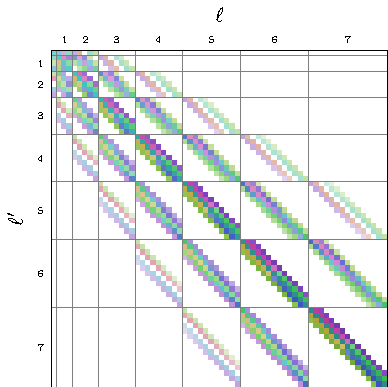
\includegraphics[width=\textwidth]{Bmat_se3_dense.pdf}
		\end{subfigure}
		\hfill
		\begin{subfigure}[b]{0.31\textwidth}
			\centering
			\caption{$\Sigma = \smqty(\dmat{\Sigma_{RR}, \Sigma_{vv}})$}
			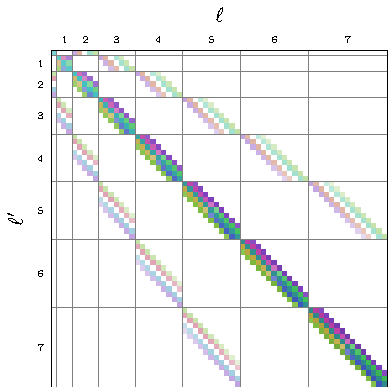
\includegraphics[width=\textwidth]{Bmat_se3_indep.pdf}
		\end{subfigure}
		\hfill
		\begin{subfigure}[b]{0.31\textwidth}
			\centering
			\caption{$\Sigma = \smqty(\dmat{0, \Sigma_{vv}})$}
			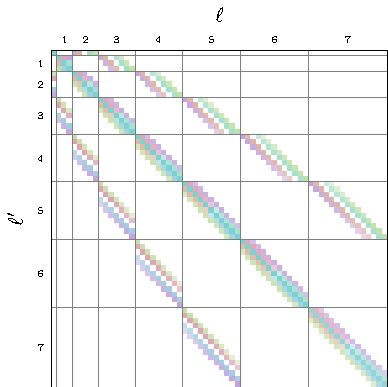
\includegraphics[width=\textwidth]{Bmat_se3_trans.pdf}
		\end{subfigure}

		\bigskip
		\begin{subfigure}[b]{0.31\textwidth}
			\centering
			\caption{$\Sigma = \smqty(\dmat{\Sigma_{RR}, 0})$}
			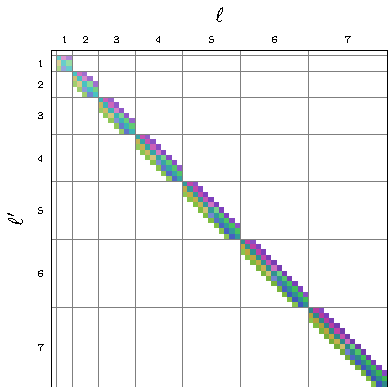
\includegraphics[width=\textwidth]{Bmat_se3_rot.pdf}
		\end{subfigure}
		\begin{subfigure}[b]{0.31\textwidth}
			\centering
			\caption{$\Sigma = \smqty(\dmat{\sigma_R^2 I_3, \sigma_v^2 I_3})$}
			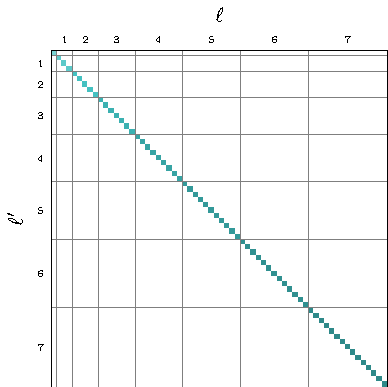
\includegraphics[width=\textwidth]{Bmat_se3_scalarindep.pdf}
		\end{subfigure}
		\caption[Structure of $B^0$ matrix for $\SE{3}$]{
			Structure of $B$ matrix for $\SE{3}$ for special cases of $\Sigma$.
			$\Sigma_{RR}$ and $\Sigma_{vv}$ are $3 \times 3$ diffusion sub-matrices for rotation and translation, respectively.
			$\sigma_R^2 I_3$ and $\sigma_v^2 I_3$ are scalar diagonal diffusion matrices.
		}
		\label{fig:bmat_se3}
	\end{figure*}

	\begin{figure*}
		\centering
		\begin{subfigure}[b]{0.31\textwidth}
			\centering
			\caption{dense $\Sigma$}
			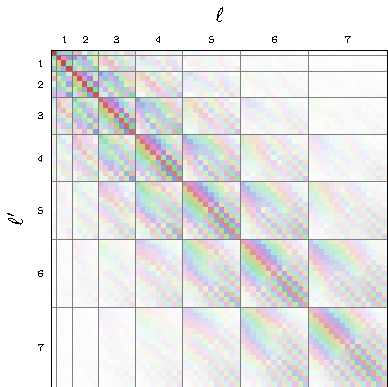
\includegraphics[width=\textwidth]{ftrans_se3_dense.pdf}
		\end{subfigure}
		\hfill
		\begin{subfigure}[b]{0.31\textwidth}
			\centering
			\caption{$\Sigma = \smqty(\dmat{\Sigma_{RR}, \Sigma_{vv}})$}
			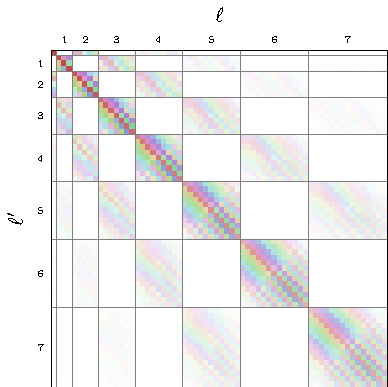
\includegraphics[width=\textwidth]{ftrans_se3_indep.pdf}
		\end{subfigure}
		\hfill
		\begin{subfigure}[b]{0.31\textwidth}
			\centering
			\caption{$\Sigma = \smqty(\dmat{0, \Sigma_{vv}})$}
			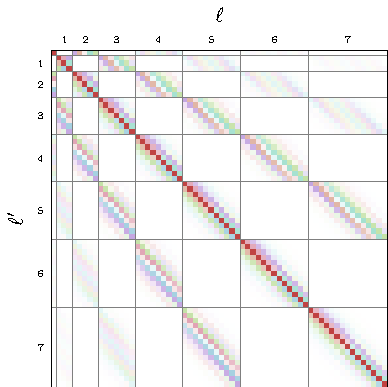
\includegraphics[width=\textwidth]{ftrans_se3_trans.pdf}
		\end{subfigure}

		\bigskip
		\begin{subfigure}[b]{0.31\textwidth}
			\centering
			\caption{$\Sigma = \smqty(\dmat{\Sigma_{RR}, 0})$}
			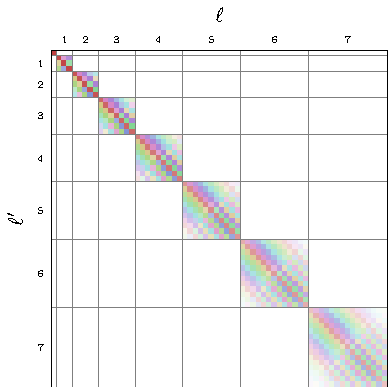
\includegraphics[width=\textwidth]{ftrans_se3_rot.pdf}
		\end{subfigure}
		\begin{subfigure}[b]{0.31\textwidth}
			\centering
			\caption{$\Sigma = \smqty(\dmat{\sigma_R^2 I_3, \sigma_v^2 I_3})$}
			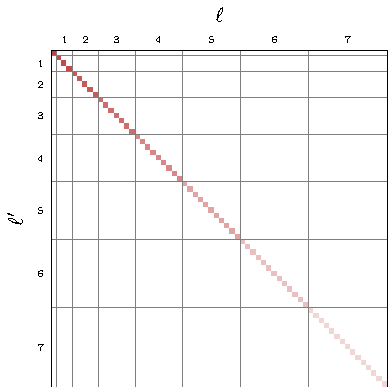
\includegraphics[width=\textwidth]{ftrans_se3_scalarindep.pdf}
		\end{subfigure}
		\caption[Structure of the diffusion normal Fourier transform for $\SE{3}$]{
			Structure of the Fourier transform $\coef{\pi}^0(1)$ for the diffusion normal distribution on $\SE{3}$ for special cases of $\Sigma$.
			$\Sigma_{RR}$ and $\Sigma_{vv}$ are $3 \times 3$ diffusion sub-matrices for rotation and translation, respectively.
			$\sigma_R^2 I_3$ and $\sigma_v^2 I_3$ are scalar diagonal diffusion matrices.
		}
		\label{fig:diffnorm_ftrans_se3}
	\end{figure*}

	There are a few additional special cases worth considering.
	First, if $\Sigma_{R} = 0$, so that there is no rotational variance, then the rotational distribution is a Dirac measure, and it is well known that the translational distribution is a trivariate normal distribution.
	On the other hand, if there is no translational variance, so that $\Sigma_v=0$. the translational distribution is not a Dirac measure, as the rotations still perturb the positions of points within each rigid body.
	The rotational distribution, however, reduces to the diffusive normal distribution on $\SO{3}$ with $\Sigma = \Sigma_R$.

	If $\Sigma = \smqty(\dmat{\sigma_R^2 I_3, \sigma_v^2 I_3})$, then using \cref{square_se3_iur_is_scalar}, $B^s$ has a block-scalar structure with elements:
	$$B^s_{\ell',m'\ell,m}(p) = - \frac{1}{2} \qty(\sigma_R^2 \ell' (\ell' + 1) + \sigma_v^2 p^2) \delta_{\ell',\ell} \delta_{m',m}.$$
	As a result, the matrix exponential of this matrix is likewise block-scalar, and we can explicitly write the elements of $\coef{\pi}$ as
	\begin{equation}
		\coef{\pi}^s_{\ell',m',\ell,m}(p) = e^{-\frac{1}{2} \sigma_v^2 p^2} e^{- \frac{1}{2} \ell' (\ell' + 1) \sigma_R^2} U^s_{\ell',m',\ell,m}(\mu^{-1}, p)
	\end{equation}
	We can make a few important observations.
	%\todo{equations, references, language}
	First, the $e^{-\frac{1}{2} \sigma_v^2 p^2}$ term is the classical Fourier transform of a zero-centered rotationally symmetric multivariate normal distribution.
	Because it contains no indices and is scalar, it commutes upon convolution.
	That is, if we convolve any other distribution with $\pi$, this term will still factor out.
	Moreover, if we convolve $\pi$ with another diffusion normal distribution with $\Sigma$ of the same structure, then the $\sigma_v$ terms compose.
	Second, the $e^{- \frac{1}{2} \ell' (\ell' + 1) \sigma_R^2}$ term arises in the expression of Brownian rotational diffusion on $\SO{3}$ \supercite{perrinEtudeMathematiqueMouvement1928}.
	If only the rotational distribution is under consideration, then we may use the Fourier transform on $\SO{3}$ of only the rotational part of the distribution:
	$$\coef{\pi}^{\ell} = e^{- \frac{1}{2} \ell (\ell + 1) \sigma_R^2} U^{\ell}(R^{-1}).$$
	Because $U(R)$ is block-diagonal, the $e^{- \frac{1}{2} \ell (\ell + 1) \sigma_R^2}$ terms commute upon convolution.
	Repeated convolution of diffusion normal distributions then results in these scalar terms collecting and the IURs composing using the group law.
	As a result, the convolution of two diffusion normal distributions on $\SE{3}$ with a $\Sigma$ of this structure produces a distribution on $\SE{3}$ whose orientational component is a diffusion normal distribution on $\SO{3}$.

	\section{Sampling from the diffusion normal distribution}

	To sample from $\diffnorm(\mu, \Sigma)$, we employ the Euler-Maruyama scheme proposed in \cite[Section IV]{wooramparkDiffusionBasedMotionPlanning2005} for $\SE{3}$, which we write with the following $n$-step sampling procedure for $i \in \{0, 1, \ldots, n\}$:
	\begin{align*}
		g_0       & = \mu                                               \\
		x_i       & \sim \mathrm{MvNormal}\qty( 0, \frac{1}{n} \Sigma ) \\
		g_{i + 1} & = g_i \circ \expm \qty( \sum_{i=1}^d x_i E_i )
	\end{align*}
	The final step $g_n$ is approximately drawn from $\diffnorm(\mu, \Sigma)$.
	Note that this is just a left-translated discretization of the stochastic differential equation defined above.
	\cite{piggottGeometricEulerMaruyama2016} performed a rigorous error analysis of the method for $\SO{n}$ and of a similar method for simulating independent diffusion of rotation and translation on $\SE{n}$; to our knowledge a rigorous error analysis of the method for the general $\SE{3}$ has not been completed.
	As $n \to \infty$, this approximation becomes exact.

	\section{The kinematic ensemble representation}\label{the-kinematic-ensemble-representation}

	A frame is some coordinate system that we can use to define relative positions and orientations.
	Given two frames $\bodyframe{F}_i$ and $\bodyframe{F}_j$, we write the rigid transformation taking $\bodyframe{F}_i$ to $\bodyframe{F}_j$ as $T_{ij} \in \SE{3}$.
	To fully specify $T_{ij}$, we need to note that it is written relative to $\bodyframe{F}_i$.
	That is, it is the transformation an observer in an unmoving $\bodyframe{F}_i$ would use to align a duplicate copy of $\bodyframe{F}_i$ to $\bodyframe{F}_j$.
	This transformation is also called a pose.
	The equivalent transformation written relative to $\bodyframe{F}_j$ is $T_{ji} = T_{ij}^{-1}$.

	% \todo{unify with main text}

	A kinematic tree representation has three components: a tree topology, a set of rigid frames, and an assignment of rigid bodies to each frame.
	The topology is a connected directed acyclic graph; in our framework, every edge is directed away from the root.
	Some nodes have children, nodes at the other end of an arrow coming out of the node.
	Conversely, each node except for the root has exactly one parent.
	The root node has no parents.
	A node's ancestor is any node along the unique path between it and the root.
	Nodes with no children are called leaves.

	The root of the tree is a unique node that represents a global reference frame $\bodyframe{O}$.
	Each node represents a frame with an implicit pose relative to $\bodyframe{O}$.
	An edge between $\bodyframe{F}_i$ and $\bodyframe{F}_j$ corresponds to the transformation $T_j = T_{ij}$, where we can drop the reference index because it is encoded in the tree topology.

	There is exactly one path between any two nodes, called a kinematic chain.
	Without loss of generality and for notational simplicity, we will consider only a single chain.
	Indexing the frames along the chain, we can write the chain $C$ as the sequence
	$$C = (\bodyframe{F}_1, \bodyframe{F}_2, \ldots, \bodyframe{F}_{n-1}, \bodyframe{F}_n).$$
	The transformation $T$ can then be written as the product of transformations along this path:
	$$T = T_{1,2} \circ T_{2,3} \circ \ldots \circ T_{n-2,n-1} \circ T_{n-1,n}.$$
	Note that if the two nodes share a common ancestor at index $k$, then rewritten in terms of transformations from parents to children only, we have:
	$$T = T_{1}^{-1} \circ T_{2}^{-1} \circ \ldots \circ T_{k-1}^{-1} \circ T_{k+1} \circ \ldots T_{n-1} \circ T_{n}.$$
	The global pose of a frame $\bodyframe{F}_{n}$ can be obtained by setting $\bodyframe{F}_1$ to be $\bodyframe{O}$.
	Consequently, all pairwise transformations and global poses are encoded in the tree structure with the set of transformations at the edges.

	A kinematic ensemble is a distribution of kinematic trees, where the topology is fixed, and only the transformations of the edges vary\footnote{
		More properly, the kinematic ensemble is a distribution on the power manifold $[\SE{3}]^n$, where $n$ is the number of edges.
	}.
	The ensemble has the same topology as its trees.
	Consequently, we can construct an ensemble by drawing the transformations from a distribution.
	Unlike transformations in the kinematic tree, we cannot easily obtain corresponding distributions on pairwise transformations between any two frames in the kinematic ensemble.

	To do so, we must assume that each transformation is conditionally independent of all other transformations, so that we can write $T_i \sim \pi_i$, and, equivalently, $T_{ij} \sim \pi_{ij}$ for all $i$ along a chain.
	The end-to-end distribution of $T$ is then
	$$
		\pi = \finversion{\pi_1} \convwith \finversion{\pi_2} \convwith
		\ldots \convwith \finversion{\pi_{k-1}} \convwith \pi_{k+1}
		\ldots \convwith \pi_{n-1} \convwith \pi_{n}
	$$

	As we have seen earlier, the Fourier transform of the density of this distribution is the reverse product of the Fourier transforms of the densities of the distributions along the chain, where for the inversions the Fourier transforms are conjugate transposed:
	\begin{equation}
		\coef{\pi}(\lambda) = \coef{\pi}_{n}(\lambda) \coef{\pi}_{n-1}(\lambda) \ldots \coef{\pi}_{k+1}(\lambda) \hconj{\coef{\pi}_{k-1}(\lambda)} \ldots \hconj{\coef{\pi}_{2}(\lambda)} \hconj{\coef{\pi}_{1}(\lambda)}
	\end{equation}
	The density of $\pi$ is obtained by Fourier inversion.

	In summary, we can compute the density of the distribution of the transformations between any two frames by computing the Fourier transform of the densities of all distributions along the chain between the frames, multiplying them, using the conjugate transpose when necessary, and then computing the inverse Fourier transform.
	All chains that include a node will use the same Fourier transform for that node; therefore, the transforms need only be computed once and then can be reused to compute the densities of many pairwise transformation distributions;
	however, in some cases it is more efficient to avoid directly computing the Fourier transforms (below).

	When representing a biological macromolecule as a kinematic ensemble, we first must partition the macromolecule into multiple rigid bodies.
	These rigid bodies will generally correspond to domains in a single molecule or subunits in a complex, and these assignments must be based on some other analysis.
	Each body is assigned a frame, giving the particles in the body local coordinates (relative to the body frame); the frame is chosen so that the atoms are distributed around the origin in this frame.
	Because the transformations between bodies are represented with distributions, it is not necessary to represent the connections between the bodies with full atomic detail; indeed, this may make sampling more difficult.
	Hence, we do not explicitly represent linkers between domains.
	A choice of distributions for each edge, parameterized by some degrees of freedom, completes the ensemble.

	In general, we can use as the edge distributions either the Dirac measure, the diffusion normal, a mixture of either of the two distributions, or a different distribution entirely.
	The choice of distribution is guided by prior information, biological intuition, direct simulation, and ability to reproduce the data.

	\section{Marginal density functions}

	From a probability density function $\pi \in L^2(\SE{3})$ expressed in terms of the Fourier transform on $\SE{3}$ using the inversion formula, we can compute several marginal density functions by integrating out certain degrees of freedom.
	While many of these have been derived in previous works, they have not all been collected in one location and related to an underlying distribution on $\SE{3}$.
	As we show, in many cases these marginal densities are expressed in terms of commonly used orthogonal bases we have previously discussed.
	As a result, efficient methods are often available for computing the densities and expectations against them.

	\subsection{Orientational density function}

	The orientational density function is the the density of the distribution of the rotation from one rigid body to another, ignoring the translational component.
	Given $\pi \in L^2(\SE{3})$, we write the orientational density with respect to the uniform measure $\dd R$ using the inverse Fourier transform on $\SO{3}$:
	\begin{equation}
		\pi(R) = \sum_{\ell=0}^\infty (2\ell+1) \sum_{m,n=-\ell}^\ell \coef{\pi}^0_{\ell,m,\ell,n}(0) U^\ell_{nm}(R) \dd R.
	\end{equation}

	\subsection{Polar density function}

	From the ODF we can compute the polar density function, the density of the distribution of the angle between a unit vector in one rigid frame and a unit vector in another rigid frame.
	If we take the first vector to be aligned with the $z$-axis in its frame, then in the $zyz$ Euler angle convention, the angle $\theta$ of the rotation $R(\phi,\theta,\psi)$ around the $y$-axis corresponds to this polar angle.
	Consequently, given $\pi \in L^2(\SO{3})$, the polar density function with respect to the measure $\sin\theta \dd\theta$ is
	\begin{align}
		\pi(\theta) & = \frac{1}{8\pi^2} \int_0^{2\pi} \int_0^{2\pi} \pi(R(\phi,\theta,\psi)) \dd\phi \dd\psi \label{polar_dens_def}             \\
		            & = \frac{1}{2} \sum_{\ell=0}^\infty (2\ell+1) \coef{\pi}^0_{\ell,0,\ell,0}(0) P_\ell(\cos\theta). \label{polar_dens_ftrans}
	\end{align}
	The terms $\coef{\pi}^0_{\ell,0,\ell,0}(0)$ are therefore the coefficients of the Fourier-Legendre series of $\pi(\theta)$.

	\subsection{Positional density function}

	Given a density function $\pi \in L^2(\SE{3})$, we can obtain the marginal density of the translation vector from the position of one rigid body to the position of second rigid body in the reference frame of the first rigid body as $$\pi(v) = \int_{\SO{3}} \pi(v, R) \dd R,$$
	for $v \in \bbR^3$ and $R \in \SO{3}$.
	In terms of the $\SE{3}$ Fourier transform, this density with respect to the Lebesgue measure $\dd v$ on $\bbR^3$ is written
	\begin{equation} \label{pos_dens}
		\pi(v) = \frac{1}{\sqrt{4\pi}} \sum_{\ell=0}^\infty \sum_{m=-\ell}^{\ell} \qty((-\im)^{\ell} \frac{2}{\pi} \int_{0}^\infty \conj{\coef{\pi}^0_{0,0,\ell,m}(p)} j_{\ell} (p \norm{v}) p^2 \dd{p}) Y^{m}_{\ell} \qty( \frac{v}{\norm{v}} ).
	\end{equation}
	This is a spherical harmonic expansion, where the coefficients of the expansion are computed using an inverse spherical Hankel transform.
	An alternative is to write $\pi(v)$ as the usual inverse Fourier transform in $\bbR^3$
	\begin{align}
		\pi(v)               & = \frac{1}{(2\pi)^3} \int_{\bbR^3} e^{\im \trans{\omega} v} \ftrans{\pi}(\omega) \dd \omega                                                                                                 \\
		\ftrans{\pi}(\omega) & = \frac{1}{\sqrt{4 \pi}} \sum_{\ell=0}^\infty \sum_{m=-\ell}^{\ell} \qty(4 \pi (-1)^{\ell} \conj{\coef{\pi}^0_{0,0,\ell,m}(\norm{\omega})}) Y^{m}_{\ell}\qty(\frac{\omega}{\norm{\omega}}),
	\end{align}
	where $\ftrans{\pi}(\omega)$ is the Fourier transform of $\pi(v)$ in $\bbR^3$ and is written in terms of a spherical harmonic expansion.
	Left- and right- convolving $\pi(v, R)$ with a pure translational Dirac measure enables computation of $\pi(v)$ for $v$ the vector between any two points in a given kinematic chain.

	\subsection{Directional density function}

	From \cref{pos_dens}, we can determine one type of directional density function, namely, the density of the distribution of the unit vector $u = \frac{v}{\norm{v}} \in \mathbb{S}^2$.
	We can write this density with respect to the un-normalized measure $\dd u$ in terms of the spherical harmonic expansion:
	\begin{align*}
		\pi(u)
		 & = \frac{1}{\sqrt{4 \pi}} \sum_{\ell=0}^\infty \sum_{m=-\ell}^{\ell} a^{m}_\ell Y^{m}_{\ell}(u), \quad a^m_\ell = (-\im)^{\ell} \int_{0}^\infty \qty( \frac{2}{\pi} \int_{0}^\infty \conj{\coef{\pi}^0_{0,0,\ell,m}(p)} j_{\ell} (p r) p^2 \dd{p}) r^2 \dd{r}
	\end{align*}

	\subsection{Radial density function}

	Alternatively, by integrating out the directional component from \cref{pos_dens}, we obtain the density of the radial (\ie distance, or end-to-end) distribution with respect to the measure $r^2 \dd r$:
	\begin{equation}\label{distance_dist_ftrans}
		\pi(r) = \int_{\mathbb{S}^2} \pi(r u) \dd{u} = \frac{2}{\pi} \int_{0}^\infty \coef{\pi}^0_{0,0,0,0}(p) j_0(r p) p^2 \dd{p}.
	\end{equation}
	This is the 0-order inverse spherical Hankel transform of $\coef{\pi}^0_{0,0,0,0}(p)$.
	The use and properties of the Hankel transform in statistics were explored in \cite{lordUseHankelTransform1954}.
	There are a number of methods to efficiently approximate the inverse transform; we describe one such approach below.

	\section{Simulating NOE measurements from kinematic ensembles}\label{simulating-data-from-kinematic-ensembles}

	To simulate nuclear Overhauser effect measurements (NOEs) from the kinematic ensemble representation, we need to compute ensemble averages over the radial density function $\pi(r)$, whose form is given in \cref{distance_dist_ftrans}, between two spin pairs.
	The ensemble average is written
	\begin{equation}
		\expect{r^{-6}}{\pi} = \int_{0}^\infty r^{-6} \pi(r) r^2 \dd{r} =  \int_{0}^\infty r^{-4} \pi(r) \dd{r}.
	\end{equation}

	To compute $\pi(r)$ and this expectation, we employ the quasi-discrete spherical Hankel transform (QDSHT), described below.

	For the ensemble average integral to converge, as $r \to 0$, $\pi(r)$ must approach 0 faster than $r^4$, and as $r \to \infty$, $r^{-4} \pi(r)$ must rapidly approach 0.
	The latter condition is generally satisfied.
	However, the the former is not in general satisfied for a continuous $\pi(r)$ and specifically is violated for $\pi(r)$ computed from a convolution of diffusion normal distributions, because with a continuous ensemble representation, it is possible even if unlikely for two spin pairs to occupy the same space.
	We therefore explicitly encode an excluded volume correction by setting $\pi(r) = 0$ for $r < r_{min}$, where $r_{min}$ is chosen to prevent overlap of the two atoms.
	When computing the expectation using QDSHT, this modification is only necessary when $r_1 < r_{min}$.

	\section[The quasi-discrete spherical Hankel transform]{Computing the expectation with the quasi-discrete spherical Hankel transform}

	The method described here draws inspiration from the quasi-discrete Hankel transform (QDHT), which was first generally introduced in \cite{johnsonImprovedMethodComputing1987}, though not yet by that name.
	For zero and integer order, detailed error analyses of the method were performed in \cite{yuQuasidiscreteHankelTransform1998,guizar-sicairosComputationQuasidiscreteHankel2004}.
	Our contribution is to generalize the technique for the spherical Hankel transform of arbitrary order.
	Furthermore, we develop a technique for approximating certain expectations against a radial density function using zeros of the spherical Bessel functions.

	Recall that for $r,p > 0$ and $f \in L^2([0, \infty))$, the spherical Hankel transform and its inverse were defined in \cref{spherical_hankel} as
	\begin{equation*}
		f(r) = \frac{2}{\pi}\int_0^\infty \coef{f}(p) j_\nu(p r) p^2 \dd p, \quad \coef{f}(p) = \int_0^\infty f(r) j_\nu(p r) r^2 \dd r.
	\end{equation*}

	Assume $f(r) = 0$ for $r > R > 0$ and $\coef{f}_\nu(p) = 0$ for $p > P > 0$.
	Then, by \cite[Eqs. 11.51 and 11.52]{arfkenMathematicalMethodsPhysicists2005}, we can expand $f(r)$ using the Fourier-Bessel series:
	\begin{align*}
		f(r)      & = \sum_{k=1}^\infty c_{\nu,k} J_{\nu}\qty(\alpha_{\nu,k} \frac{r}{R})                                        \\
		c_{\nu,k} & = \frac{2}{R^2 J_{\nu + 1}(\alpha_{\nu,k})^2} \int_0^R f(r) J_{\nu}\qty(\alpha_{\nu,k} \frac{r}{R}) r \dd r,
	\end{align*}
	where $\alpha_{\nu,k}$ is the $k$th positive root of $J_\nu$, (\ie $J_\nu(\alpha_{\nu,k}) = 0$ and $\alpha_{\nu,k} > 0$).
	By reparameterization, we can write an equivalent spherical Fourier-Bessel series:
	\begin{align*}
		f(r)      & = \sum_{k=1}^\infty c_{\nu,k} j_{\nu}\qty(\alpha_{\nu,k} \frac{r}{R})                                          \\
		c_{\nu,k} & = \frac{2}{R^3 j_{\nu + 1}(\alpha_{\nu,k})^2} \int_0^R f(r) j_{\nu}\qty(\alpha_{\nu,k} \frac{r}{R}) r^2 \dd r,
	\end{align*}
	where now $\alpha_{\nu,k}$ is the $k$th positive root of $j_\nu$.
	Note that $c_{\nu,k} = \frac{2}{R^3 j_{\nu + 1}(\alpha_{\nu,k})^2} \coef{f}_{\nu}\qty(\frac{\alpha_{\nu,k}}{R})$.
	Thus, letting $p_k = \frac{\alpha_{\nu,k}}{R}$ and $r_i = \frac{\alpha_{\nu,i}}{P}$,
	$$f(r_i) = \frac{2}{R^3} \sum_{k=1}^\infty \frac{j_{\nu}\qty(r_i p_k)}{j_{\nu + 1}(R p_k)^2} \coef{f}_{\nu}\qty(p_k).$$
	So far, this is exact.
	The quasi-discrete approach is to truncate the series at some large $k=K$ and choose $R P = \alpha_{\nu, K + 1}$.
	Then, we can write the inverse of the quasi-discrete spherical Hankel transform (QDSHT) of order $\nu$ as
	\begin{equation}\label{qdsht_inverse}
		f(r_i) \approx \sum_{k=1}^K T_{ik} \coef{f}_{\nu}(p_k), \quad T_{ik} = \frac{2}{R^3} \frac{j_{\nu}\qty(\frac{\alpha_{\nu,i} \alpha_{\nu,k}}{\alpha_{\nu,K+1}})}{j_{\nu + 1}(\alpha_{\nu,k})^2},
	\end{equation}
	where $T$ is a precomputed matrix of size $(K, K)$.
	A similar approach yields the forward QDSHT:
	\begin{equation}\label{qdsht}
		\coef{f}_\nu(p_k) = \frac{\pi}{P^3} \sum_{i=1}^\infty \frac{j_\nu(r_i p_k)}{j_{\nu+1}(P r_i)} f(r_i) \approx \frac{\pi}{2} \qty(\frac{R}{P})^3 \sum_{i=1}^K T_{ki} f(r_i),
	\end{equation}
	where the matrix $T$ is the same as that used in the inverse QDSHT.
	Note that both the forward and reverse transform contain a multiplication by the matrix $T$; only the scalar normalization factor is different.

	By specifying a large $R$ above which $\pi(r)$ should be zero, a large $K$, and $\nu=0$, this method then determines the values $p_k$ at which we must evaluate $\coef{\pi}_{0,0,0,0}^0(p_k)$.
	We then could use this matrix-vector product to compute the $\pi(r_i)$ values in $\order{K^2}$ operations.
	However, our goal is not to compute $\pi(r_i)$.
	We instead need to approximate an integral of the form $\int_0^R f(r) r^2 \dd r$, where $f(r) = g(r) \pi(r)$ (\eg in our case $g(r) = r^{-6}$).
	Assume for the moment that $f \in L^2([0, \infty))$; this condition can be ensured in our case by truncating at a minimum value of $r_i$.
	Then $\coef{f}_0(0) = \int_0^\infty f(r) j_0(0) r^2 \dd r = \int_0^\infty f(r) r^2 \dd r$.
	Thus, we only need to approximate $\coef{f}_0(0)$.
	Using \cref{qdsht}, the solution is
	$$\coef{f}_0(0) = \frac{\pi}{P^3} \sum_{i=1}^\infty \frac{g(r_i)}{j_{1}(P r_i)^2} \pi(r_i) \approx \frac{\pi}{P^3} \sum_{i=1}^K \frac{g(r_i)}{j_{1}(P r_i)^2} \pi(r_i).$$
	In principle, we could then compute $\pi(r_i)$ using the inverse QDSHT and then use this equation to approximate the integral.
	However, it is more efficient to fuse the two steps:
	\begin{equation}
		\begin{gathered}
			\int_0^\infty g(r) \pi(r) r^2 \dd r \approx \sum_{k=1}^K \beta_k \coef{\pi}_{0,0,0,0}^0(p_k) \\
			\beta_k = \frac{2\pi}{\alpha_{0,K+1}^3} j_{1}(\alpha_{0,k})^{-2} \sum_{i=1}^K j_0\qty(\frac{\alpha_{0,i} \alpha_{0,k}}{\alpha_{0,K+1}}) j_{1}(\alpha_{0,i})^{-2} g(r_i).
		\end{gathered}
	\end{equation}
	The vector $\beta$ is entirely determined by $R$, $K$, and the function $g$ and is therefore computed once and re-used for every integral.
	As a result, the complexity of approximating the integral scales with $\order{K}$.

	\section{Implementation notes}

	Here we describe several challenges to efficient implementation of the kinematic ensemble approach and some solutions.
	If implemented naively, the storage and time complexity can be quite large.
	For example, each $\ell$ block of a Wigner $D$-matrix is of dimension $(2\ell+1,2\ell+1)$, thus having $\order{\ell^2}$ elements.
	Computing all entries to a maximum value $L \ge \ell$, the number of entries is then $\order{L^3}$; hence even an algorithm like the recurrence relations of \cite{choiRapidStableDetermination1999}, which computing the entries in linear time, still will have a time and storage complexity of $\order{L^3}$.
	Given two matrices with the block-diagonal structure of the IURs of $\SO{3}$, the product of those matrices occurs block-wise.
	Multiplication of each block is $\order{\ell^3}$, while multiplication of all blocks in the worst case is $\order{L^4}$.
	The matrix exponentiation necessary to compute the Fourier transform of the density of the diffusion normal distribution has the same time complexity, with a higher constant factor.
	Thus, for large $L$, each scoring function evaluation can be very expensive.

	The situation is worse for $\SE{3}$, even if we limit ourselves to the $s=0$ blocks, the only blocks we use here.
	First, the IURs are not block sparse; hence for maximum $L$, the $s=0$ block has a size $((L+1)^2,(L+1)^2)$, with $\order{L^4}$ entries.
	In general these entries cannot be computed in linear time, and the worst-case complexity of computing all entries is $\order{L^5}$.
	Multiplication of the blocks is $\order{L^6}$, and matrix exponentiation has the same time complexity.
	Moreover, most operations need to be repeated for multiple $p_k$; hence, for $M$ kinematic chains, $N$ the number of nodes in the longest chain, and $K$ the number of grid points $p_k$ sampled for QDSHT, the time complexity of the scoring function is then $\order{N M K L^6}$.

	For large $L$ and $P$, this complexity makes the scoring function infeasible for sampling with MCMC.
	However, we can obtain a much better time complexity by noting that we do not need the matrix $\coef{\pi}(p_k)$.
	We only need a single element $\coef{\pi}^0_{0,0,0,0}(p_k)$.
	We can compute this element as
	$$\coef{\pi}^0_{0,0,0,0}(p_k) = \sum_{\ell'=0}^L \sum_{m'=-\ell'}^{\ell'} \sum_{\ell=0}^L \sum_{m=-\ell}^{\ell} \delta_{\ell',0} \delta_{m',0} \coef{\pi}^0_{\ell',m',\ell,m}(p_k) \delta_{\ell,0} \delta_{m,0}.$$
	But this is just left- and right-multiplication of the Fourier transform matrix by a one-hot vector $v = \trans{\qty(1, 0, 0, \ldots)}$ with a single non-zero element:
	$$\coef{\pi}^0_{0,0,0,0}(p_k) = \trans{v} \coef{\pi}^0 v = \trans{v} \qty(\coef{\pi}^0 v).$$
	Instead of explicitly computing the matrix product of Fourier transform matrices,
	$$\coef{\pi}^0(p_k) = \qty(\coef{\pi_K})^0(p_k) \cdot \ldots \cdot \qty(\coef{\pi_1})^0(p_k),$$
	we recursively compute the matrix-vector products for $j \in \{1, \ldots, J\}$:
	\begin{align*}
		w_0 & = v                                     \\
		w_j & = \qty(\coef{\pi_{j}})^0(p_k) w_{j - 1} \\
		\coef{\pi}^0_{0,0,0,0}(p_k)
		    & = \trans{v} w_J.
	\end{align*}
	For large $L$ we use another optimization.
	The $\SE{3}$ IURs $U^s(R, p_k)$ can be computed as matrix exponentials of their tridiagonal block-tridiagonal Lie algebra representations $u^s(E_k, p_k)$.
	Likewise, the Fourier transform of the diffusion normal distribution is computed as the matrix exponential of the pentadiagonal block-pentadiagonal matrix $B^s$.
	For large $L$, it is much more efficient to compute the action of the matrix exponential upon the vector $w$ instead of the exponential followed by the matrix-vector-product.
	The action of the exponential is a common operation in exponential integrators, and efficient methods like the Krylov subspace method have been developed for this purpose \supercite{al-mohyComputingActionMatrix2011}.
	The time complexity of the action of the exponential is on the order of the matrix-vector product itself, so this reduces the time complexity of scoring function evaluation to $\order{NMKL^4}$.
	Due to the block-sparse structure of the $u^s$ and $B^s$ matrices, this also substantially reduces the storage requirements of the method.
	Moreover, the method could potentially be made more efficient by leveraging the banded structure of the $u$ and $B$ matrices.
	For density functions that are not informed by translational degrees of freedom, such as the angular density above, it is sufficient to use the $u$ and $B$ matrices for $\SO{3}$, and the time complexity reduces to $\order{NML^3}$.

	For low $L$ and in particular for high $M$, however, directly evaluating the matrix exponential for a node and reusing it for all chains that pass through that node is more efficient than computing the action of the exponential multiple times.
	Moreover, as shown earlier, for some structures of diffusion matrices $\Sigma$, the Fourier transform is highly structured.
	Through extensive profiling, we have determined a number of heuristics for switching between different strategies for computing the NOE forward model.
	The method is implemented in Julia, a dynamically typed, "just-ahead-of-time" compiled language \supercite{Julia-2017}.
	Julia permits us to encode information about the structure of $\Sigma$, $u$, and $B$ into custom array types, which are then used to dispatch to optimized implementations of the forward model for a particular kinematic ensemble.

	To compute gradients, we use source-to-source reverse-mode automatic (or algorithmic) differentiation (AD) provided by the package Zygote \supercite{innesDonUnrollAdjoint2019}.
	Reverse-mode AD is a family of algorithms for computing the gradient of a function by performing a forward pass while storing intermediates, followed by a backward pass that pulls back (or back-propagates in machine learning terminology) an adjoint derivative, that is, a derivative of the scalar output of the function with respect to some intermediate \supercite{griewankEvaluatingDerivativesPrinciples2008}.
	For a function with a single output, when the adjoint is pulled back to the inputs of the function, the result is the gradient at the specific value of those inputs.
	Reverse-mode AD is linear in the time complexity of the number of outputs of a function; while in principle the gradient can be computed with less than 5 times the number of operations as the forward evaluation of the function, poor implementation or large memory requirements can increase the wall-clock time of evaluation by orders of magnitude.
	Zygote works by rewriting the source code of the function to return both the output of the function as well as a pullback function that computes the gradient.
	These functions can then be integrated into a statistical model in a probabilistic programming language.

	Where necessary, we implement custom AD rules for functions identified by profiling to have particularly poor performance when differentiated by Zygote.
	\cref{ad-rules} describes an algorithm for deriving such rules for functions with complex inputs and outputs, while \cref{ad-power-series} uses the approach to present an AD rule for a class of functions of Hermitian matrices, including the matrix exponential.
	We employ this rule in the low $L$ regime to pull back adjoint derivatives through the computation of the Fourier transform of the density of the diffusion normal distribution to the centroid $\mu$ and diffusion matrix $\Sigma$.

	\section{Prior for kinematic ensemble inference}

	Here we present the prior terms of our posterior distribution.
	For the $\gamma$ and $\sigma$ terms in the likelihood, we use weakly informative half-$t$ distributions with degrees of freedom $\nu=30$ and scale parameter of 1\footnote{
		Note that \cite{riepingInferentialStructureDetermination2005} used a Jeffreys prior for these terms.
		We do not use Jeffreys priors, however, because they are improper (\ie have infinite probability mass) and thus have poor geometric properties for sampling.
		Moreover, we cannot draw samples from them to check model assumptions.
		The priors used here have heavier tails than a half-Normal distribution and thus are weakly informative.}.
	The degrees of freedom of each diffusion normal distribution $i$ are the centroid transformation $\mu_i = (v_i, R_i)$, where $R_i$ is a rotation and $v_i$ is a translation, and a $6 \times 6$ positive semidefinite diffusion matrix $\Sigma_i$.
	Each rotation is represented as a unit quaternion $q_i$ (\ie points in the 3-sphere $\mathbb{S}^3$), so that $R_i = R(q_i)$.
	Instead of sampling $q_i$ directly, we sample a standard multivariate normally distributed vector $x_i \in \bbR^4$.
	Upon normalization, this vector is uniformly distributed on $\mathbb{S}^3$.
	We apply to each translation a broad trivariate normal prior of with standard deviation of 1000 (interpreted as in angstroms).
	This prior is effectively a smooth boundary restraint around the identity translation.
	Each diffusion matrix is factorized as $\Sigma_i = D_i K_i D_i$, where $K_i$ is a correlation matrix, and $D_i$ is a diagonal matrix of "standard deviations."
	The diagonal of $D_i$ contains the vector of rotational standard deviations $\rho_i$ and the vector of translational standard deviations $\tau_i$.
	$\rho_i$ is interpreted as in units of radians and is restrained with a half-Normal prior with a scale corresponding to $20^\circ$ in radians.
	$\tau_i$ is interpreted as in units of angstroms and is restrained and with a half-Normal prior with scale of 10.
	The correlation matrix $K$ is restrained with an LKJ prior with a shape parameter of 2, which is effectively a uniform prior on the space of correlation matrices\supercite{lewandowskiGeneratingRandomCorrelation2009}.

	The prior is written succinctly as
	\begin{align}
		\begin{split}
			\gamma   & \sim \mathrm{StudentT}(\sigma=1, \nu=30), \quad \gamma > 0                                          \\
			\sigma   & \sim \mathrm{StudentT}(\sigma=1, \nu=30), \quad \sigma > 0                                          \\
			x_i &\sim \mathrm{MvNormal}(\mu=0, \Sigma=I_4)\\
			q_i &= \frac{x_i}{\norm{x_i}}\\
			v_i      & \sim \mathrm{MvNormal}(\mu = 0, \Sigma = \qty(10^3)^2 I_3)                                           \\
			\mu_i    & = (v_i, R(q_i))                                                                                      \\
			\rho_i   & \sim \mathrm{MvNormal}(\mu=0, \Sigma=\qty(20 \cdot \frac{\pi}{180})^2 I_3), \quad \qty(\rho_i)_j > 0 \\
			\tau_i   & \sim \mathrm{MvNormal}(\mu=0, \Sigma=10^2 I_3), \quad \qty(\tau_i)_j > 0                             \\
			D_i      & = \diag\mqty(\rho_i \\ \tau_i) \\
			K_i      & \sim \mathrm{LKJ}(2)                                                                                 \\
			\Sigma_i & = D_i K_i D_i                                                                                              \\
		\end{split}
	\end{align}

	\clearpage
	\printbibliography[heading=subbibintoc]
\end{refsection}

\end{document}